\chapter{Results and Discussion}

\section{Experimentation Environment Set Up}

All experiments reported in this chapter were produced by a single command, \code{python -m compiler.main --benchmark-all}, which compiles each of the fifteen benchmark programs under all 721 orderings, interprets every result, and writes the metrics, plots, and geometric-mean summary. The command is deterministic: the compiler uses no randomness, no timing, and no floating-point arithmetic in any decision, so repeated runs on any machine produce byte-identical intermediate code, assembly, and metric tables. The interactive results in Section~\ref{sec:gui} were produced by the same modules through the web application.

\begin{itemize}
  \item \textbf{Reference machine:} AMD Ryzen 7 7435HS (8 cores, 16 threads), 24 GB RAM, solid-state storage.
  \item \textbf{Operating system:} Linux Mint 22.2 (kernel 6.17). The system was also exercised on Windows during development; results are identical.
  \item \textbf{Runtime:} Python 3.12.3; NumPy 1.26.4; matplotlib 3.11.0; FastAPI 0.141.1; Uvicorn 0.52.1; Pydantic 2.13.4; pytest 9.1.1.
  \item \textbf{Front end build:} Node.js 20, Vite 8, TypeScript 6, React 19; the built bundle is committed and was served unchanged.
  \item \textbf{Browser for screenshots:} Chromium, 1440 $\times$ 900 viewport at 2$\times$ device scale.
  \item \textbf{Repository state:} commit \code{bce09e6} (6 August 2026) of the project repository, 54 commits, all 185 tests passing.
\end{itemize}

The exhaustive benchmark of all fifteen programs, 10{,}815 compile-and-execute runs plus plot generation, completed in 23.5 seconds. Per-program times range from 0.17 seconds for \code{gcd} to 5.21 seconds for \code{2mm}, the largest program at 252 baseline instructions and 5{,}259 executed instructions; the time is dominated by interpreting the 721 optimized programs, not by optimizing them. The full test suite completed in 3.98 seconds.

\section{Functional Requirements Results Achieved}

All twelve functional requirements defined in Chapter 3 were achieved. Table~\ref{tab:fr-status} records the status of each together with the evidence that establishes it.

\begin{table}[!htb]
\centering\small
\caption{Functional Requirements Status Table}
\label{tab:fr-status}
\begin{tabular}{L{1.4cm} L{5.0cm} L{1.6cm} L{5.2cm}}
\toprule
\textbf{FR} & \textbf{Functional requirement} & \textbf{Status} & \textbf{Evidence}\\
\midrule
FR-1 & Lexical analysis with positions and comment handling & Achieved & \code{TestLexer} (12 cases); Tokens tab in Playground\\
FR-2 & Recursive-descent parsing with precedence and located errors & Achieved & \code{TestParser}, \code{TestElseIf}, \code{TestForLoop}; AST tab\\
FR-3 & Semantic analysis collecting all violations & Achieved & \code{TestSemanticAnalyzer} (14 cases); editor underlines\\
FR-4 & Three-address code generation incl.\ arrays, globals, short-circuit & Achieved & \code{TestIRGenerator}, \code{TestArrays}, \code{TestGlobals}, \code{TestShortCircuit}\\
FR-5 & IR interpretation with dynamic counts and step limit & Achieved & \code{TestInterpreter} (9 cases)\\
FR-6 & Six correct, reorderable passes & Achieved & pass unit tests (33 cases); output equality on 10{,}815 runs\\
FR-7 & Pass manager with validation and full enumeration & Achieved & \code{TestPassManager}; 721 orderings per program\\
FR-8 & Static size, cycle estimate, category breakdown & Achieved & \code{TestMetrics} (6 cases)\\
FR-9 & Exhaustive benchmark with plots and geomean & Achieved & 91 plots and summary table generated; Section~\ref{sec:empirical}\\
FR-10 & RISC-V RV32IM generation with line mapping & Achieved & \code{TestRiscvBackend} (9 cases); all benchmarks match interpreter in simulator\\
FR-11 & Interactive web application (five pages) & Achieved & \code{test\_web.py} (24 cases); Section~\ref{sec:gui}\\
FR-12 & Command-line interface & Achieved & all flags exercised in this chapter\\
\bottomrule
\end{tabular}
\end{table}

\subsection*{Empirical results of the phase-ordering study}
\label{sec:empirical}

The remainder of this section presents the results that FR-9 produces, which are the scientific content of the project.

\subsubsection*{Effect of the best ordering on each program}

Table~\ref{tab:per-program} gives, for every program, the baseline metrics and the metrics of the best ordering, and \fig{fig:reduction-by-program} shows the reductions graphically. The best ordering is the same for every program: \ordering{CF $\to$ CSE $\to$ CP $\to$ DCE $\to$ SR $\to$ AS}, or any of the 29 other orderings equivalent to it (see below). It minimizes all three metrics simultaneously on all fifteen programs; there is no program on which the smallest code is not also the cheapest code.

\begin{table}[!htb]
\centering\small
\caption{Baseline and best-ordering metrics for each program}
\label{tab:per-program}
\begin{tabular}{L{1.7cm} C{0.9cm} C{0.9cm} C{1.15cm} C{0.95cm} C{0.95cm} C{1.15cm} C{1.05cm} C{1.05cm} C{1.15cm}}
\toprule
 & \multicolumn{3}{c}{\textbf{Static size}} & \multicolumn{3}{c}{\textbf{Est.\ cycles}} & \multicolumn{3}{c}{\textbf{Dynamic count}}\\
\cmidrule(lr){2-4}\cmidrule(lr){5-7}\cmidrule(lr){8-10}
\textbf{Program} & base & best & red.\ \% & base & best & red.\ \% & base & best & red.\ \%\\
\midrule
factorial & 40 & 16 & 60.0 & 81 & 55 & 32.1 & 81 & 53 & 34.6\\
isqrt & 50 & 27 & 46.0 & 153 & 120 & 21.6 & 347 & 294 & 15.3\\
bitcount & 33 & 19 & 42.4 & 88 & 74 & 15.9 & 354 & 235 & 33.6\\
fibonacci & 22 & 13 & 40.9 & 35 & 26 & 25.7 & 236 & 189 & 19.9\\
collatz & 42 & 26 & 38.1 & 113 & 97 & 14.2 & 4{,}712 & 3{,}193 & 32.2\\
sha\_mix & 106 & 68 & 35.8 & 255 & 217 & 14.9 & 2{,}522 & 1{,}897 & 24.8\\
jacobi1d & 76 & 50 & 34.2 & 139 & 102 & 26.6 & 1{,}064 & 755 & 29.0\\
jacobi2d & 144 & 95 & 34.0 & 251 & 166 & 33.9 & 2{,}787 & 2{,}053 & 26.3\\
power & 71 & 47 & 33.8 & 202 & 178 & 11.9 & 511 & 378 & 26.0\\
gcd & 21 & 14 & 33.3 & 51 & 44 & 13.7 & 45 & 35 & 22.2\\
gemm & 164 & 119 & 27.4 & 268 & 211 & 21.3 & 3{,}081 & 2{,}591 & 15.9\\
2mm & 252 & 185 & 26.6 & 401 & 316 & 21.2 & 5{,}259 & 4{,}420 & 16.0\\
gesummv & 106 & 78 & 26.4 & 180 & 144 & 20.0 & 1{,}487 & 1{,}207 & 18.8\\
atax & 101 & 78 & 22.8 & 157 & 134 & 14.6 & 1{,}448 & 1{,}261 & 12.9\\
bicg & 94 & 73 & 22.3 & 159 & 134 & 15.7 & 1{,}283 & 1{,}082 & 15.7\\
\midrule
\textbf{Geometric mean ratio} & & & \textbf{0.6426} & & & \textbf{0.7950} & & & \textbf{0.7679}\\
\bottomrule
\end{tabular}
\end{table}

\begin{figure}[!htb]
\centering
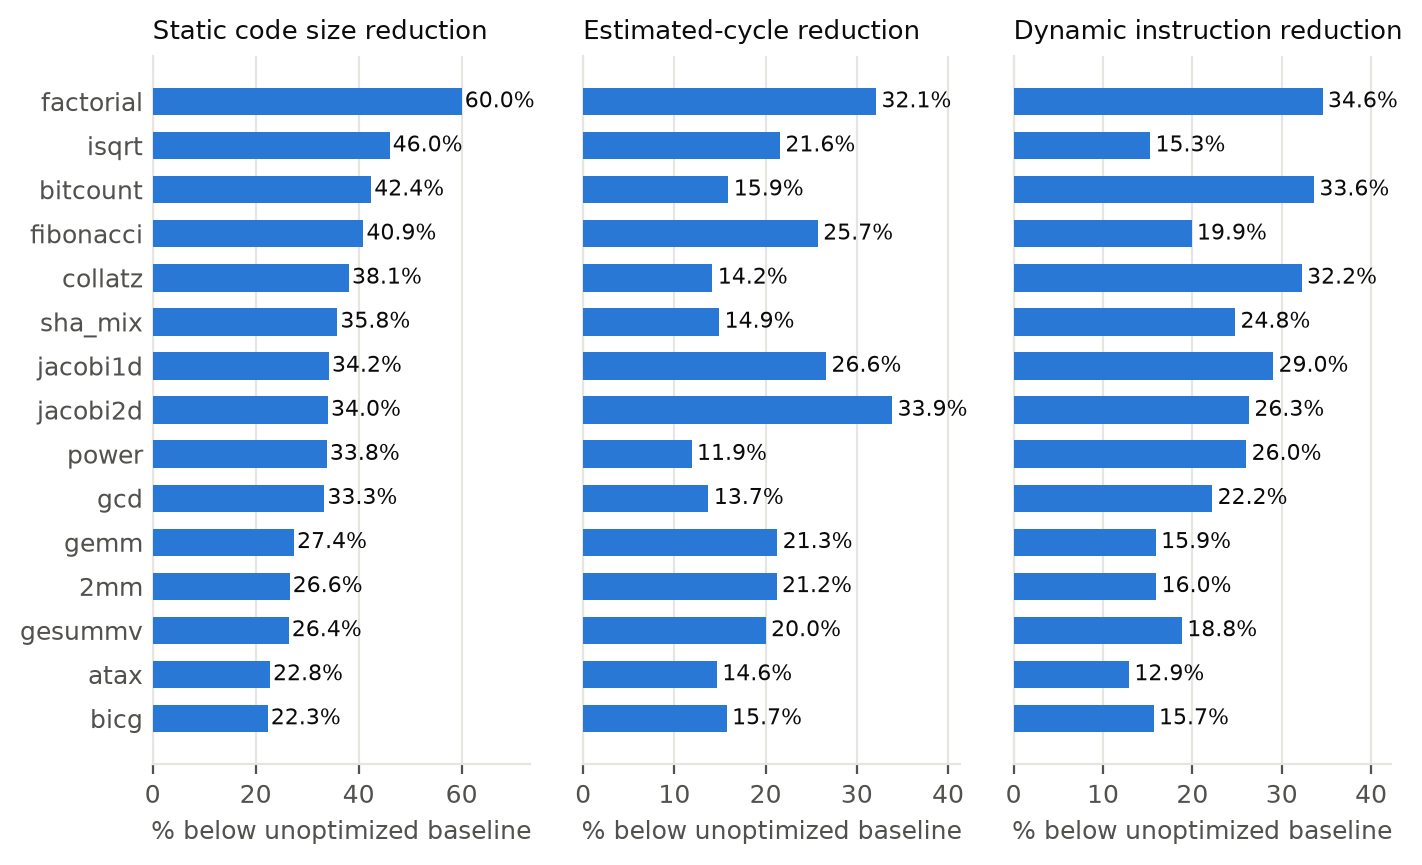
\includegraphics[width=\textwidth]{fig_reduction_by_program}
\caption[Reductions achieved by the best ordering on each program.]{Reductions achieved by the best ordering on each program, relative to the unoptimized baseline, for the three metrics. Programs are sorted by code-size reduction. The eight scalar MiBench-derived kernels occupy the top of the size ranking; the seven array-based PolyBench-derived kernels occupy the bottom.}
\label{fig:reduction-by-program}
\end{figure}

Across the fifteen programs the best ordering reduces static code size by a geometric mean of 35.7\%, the estimated cycle cost by 20.5\%, and the dynamic instruction count by 23.2\%. The size reduction ranges from 22.3\% on \code{bicg} to 60.0\% on \code{factorial}. Two groups are visible. The scalar MiBench-derived programs are reduced by 33\% to 60\% in size; the array-based PolyBench-derived programs by 22\% to 34\%. The reason is structural. In the scalar kernels, a large fraction of the baseline instructions are temporaries that hold literals (\code{t4 = 1} before \code{t5 = i + t4}) or copies from temporaries into named variables (\code{result = t0}); constant folding and copy propagation make those temporaries unread and dead code elimination removes them. In the array kernels, the loop bodies are dominated by array loads and stores and by index arithmetic on loop variables that are reassigned every iteration. Neither can be removed: memory operations are never deleted without alias analysis, and a variable that is assigned more than once is not a candidate for constant propagation. What remains removable in those kernels is the same class of literal-holding temporaries, which is a smaller share of the whole.

The cycle reductions are smaller than the size reductions everywhere except \code{jacobi2d}, and are smallest on the division-heavy programs \code{power} (11.9\%) and \code{gcd} (13.7\%). Division and modulo cost twelve cycles each in the model and are never eliminated, since their operands are loop-carried, so they dominate the cycle estimate before and after optimization. The dynamic reductions are large on the loop-heavy scalar programs (\code{bitcount} 33.6\%, \code{collatz} 32.2\%) because a single instruction removed from a loop body is removed from every iteration.

\fig{fig:box} shows the distribution of code-size reduction across all 720 orderings for each program. The boxes are narrow because most orderings fall into a few classes; the whiskers reach zero on thirteen programs because the worst orderings achieve nothing at all.

\begin{figure}[!htb]
\centering
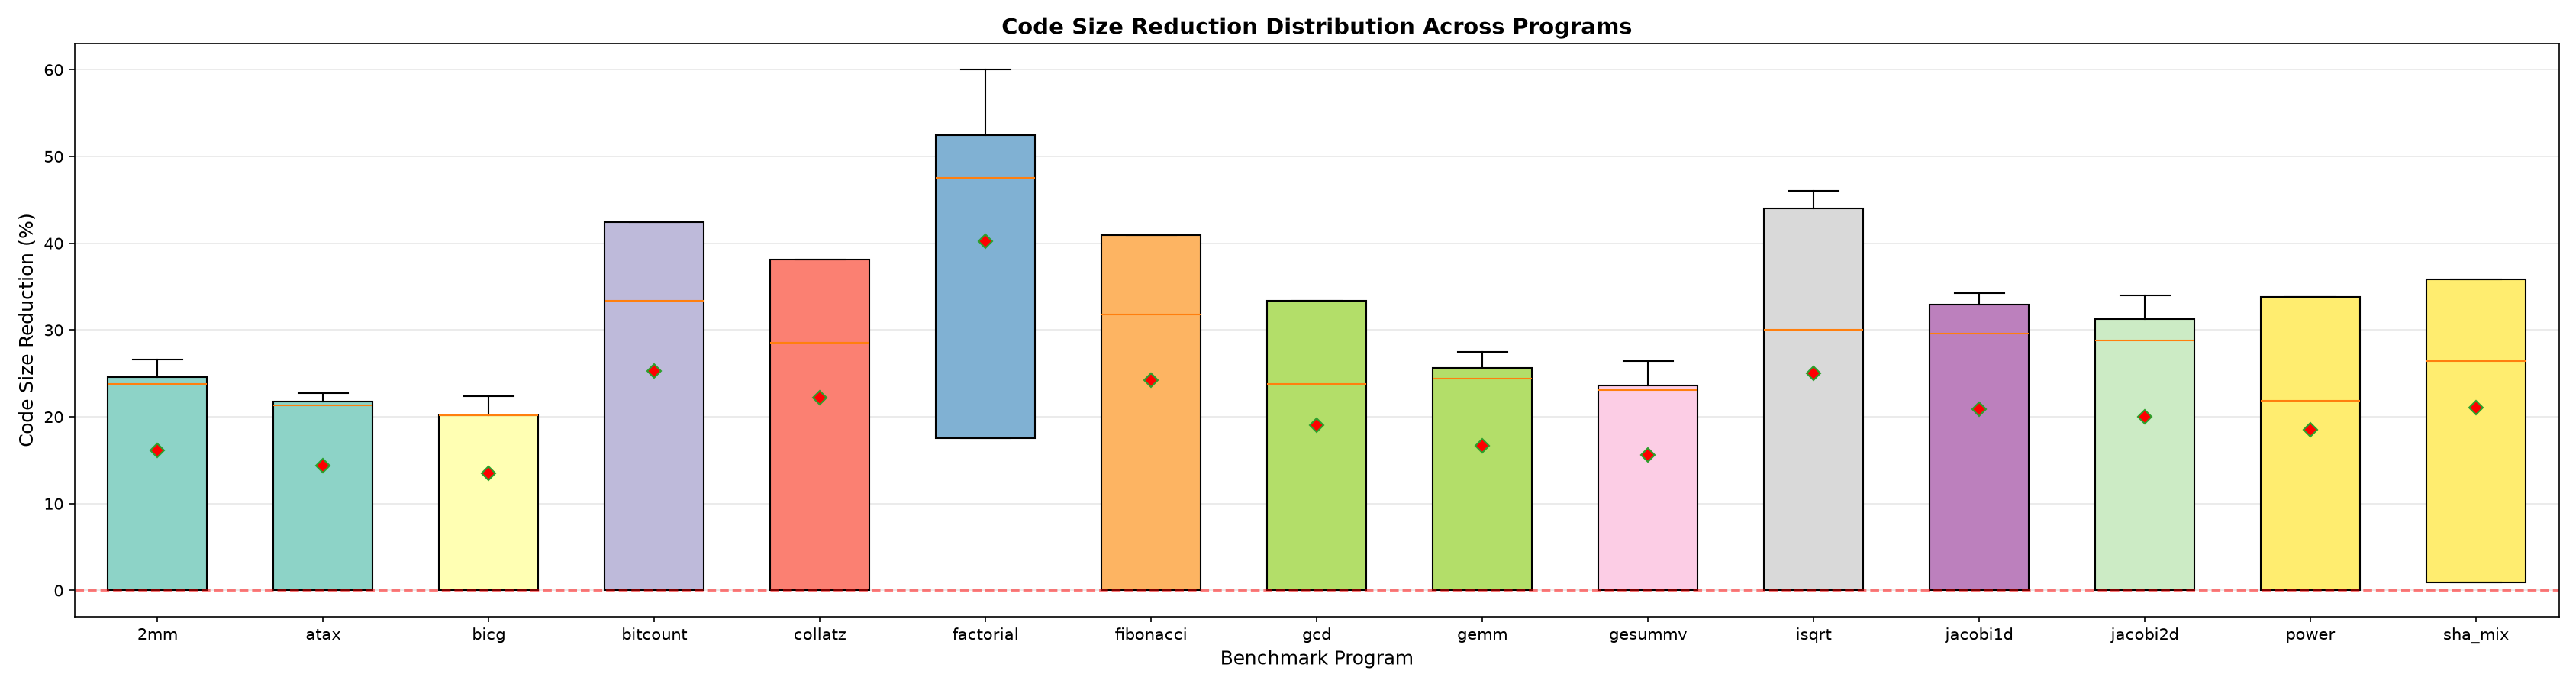
\includegraphics[width=\textwidth]{cross_program_box}
\caption[Distribution of code-size reduction across all 720 orderings, per program.]{Distribution of code-size reduction across all 720 orderings for each program, produced by the visualizer. Red diamonds mark the mean. The lower whisker touches zero on every program except \code{factorial} and \code{sha\_mix}, the two programs with planted dead code that DCE can remove without help.}
\label{fig:box}
\end{figure}

\subsubsection*{Aggregate effect of every ordering}

Aggregating with the geometric mean over the fifteen programs, the 720 orderings produce only nine distinct code-size outcomes, listed in Table~\ref{tab:classes} and plotted in \fig{fig:geomean-classes}. Each outcome is an \emph{equivalence class} of orderings that produce identical code on every program. The classes are determined entirely by the relative order of four passes, constant folding, common subexpression elimination, copy propagation, and dead code elimination; the positions of strength reduction and algebraic simplification are irrelevant to code size. The $4! = 24$ relative orders of the four passes each contain $720/24 = 30$ orderings, and the 24 relative orders map onto nine size classes, which is why the class sizes in the table are multiples of 30.

\begin{table}[!htb]
\centering\small
\caption{The nine equivalence classes of orderings, by geometric-mean normalized code size}
\label{tab:classes}
\begin{tabular}{C{0.7cm} L{6.3cm} C{1.2cm} C{1.1cm} C{1.7cm} C{1.2cm}}
\toprule
\textbf{Class} & \textbf{Relative order of CF, CSE, CP, DCE (one representative)} & \textbf{Orderings} & \textbf{Size ratio} & \textbf{Cycle ratio (range)} & \textbf{Dynamic ratio}\\
\midrule
1 & CF $\to$ CSE $\to$ CP $\to$ DCE & 30 & 0.6426 & 0.7950--0.7999 & 0.7679\\
2 & CSE $\to$ CF $\to$ CP $\to$ DCE & 30 & 0.6459 & 0.7984--0.8033 & 0.7729\\
3 & CF $\to$ CP $\to$ CSE $\to$ DCE (and CF, CP, DCE, CSE) & 60 & 0.6507 & 0.8006--0.8055 & 0.7820\\
4 & CSE $\to$ CP $\to$ CF $\to$ DCE & 30 & 0.6526 & 0.8007--0.8056 & 0.7750\\
5 & CP $\to$ CF $\to$ CSE $\to$ DCE (and two others with CP first, DCE after CF) & 90 & 0.6598 & 0.8039--0.8099 & 0.7850\\
6 & CSE $\to$ CP $\to$ DCE $\to$ CF & 30 & 0.6844 & 0.8179--0.8227 & 0.7866\\
7 & CP $\to$ CSE $\to$ DCE $\to$ CF (and two others with CP first, DCE before CF) & 90 & 0.6913 & 0.8210--0.8269 & 0.7965\\
8 & CF $\to$ CSE $\to$ DCE $\to$ CP (and three others in which CF precedes DCE and DCE precedes CP) & 120 & 0.7526 & 0.8393--0.8456 & 0.8147\\
9 & DCE before both CF and CP (eight relative orders) & 240 & 0.9866 & 0.9615--0.9675 & 0.9940\\
\midrule
 & Baseline (no optimization) & 1 & 1.0000 & 1.0000 & 1.0000\\
\bottomrule
\end{tabular}
\end{table}

\begin{figure}[!htb]
\centering
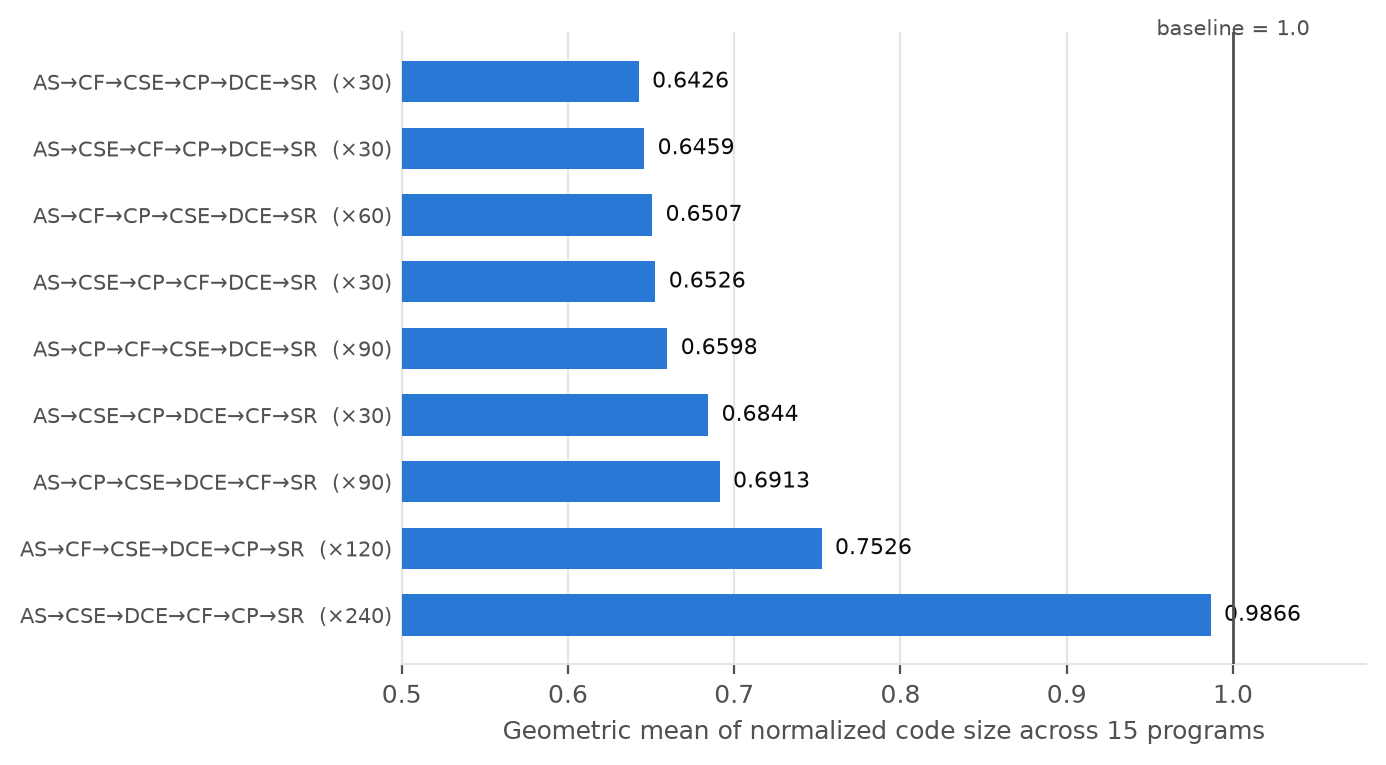
\includegraphics[width=0.95\textwidth]{fig_geomean_classes}
\caption[Geometric-mean normalized code size of the nine ordering classes.]{Geometric-mean normalized code size of the nine ordering classes, each labelled with one representative ordering and the number of orderings in the class. A third of all orderings (240) fall in the worst class and reduce code size by only 1.3\%.}
\label{fig:geomean-classes}
\end{figure}

The table reads as a set of rules. \textbf{Rule 1: DCE must come after CF and CP.} The eight relative orders in which DCE precedes both constant folding and copy propagation form class 9, a third of the whole space, with a size ratio of 0.9866: on thirteen of the fifteen programs these orderings leave the code completely unchanged, and the 1.3\% they do achieve comes entirely from the dead code planted in \code{factorial} and \code{sha\_mix}. DCE removes only instructions whose results are unread, and in the baseline IR every temporary is read at least once; it is constant folding and copy propagation that make temporaries unread, and DCE cannot benefit from what has not yet happened. \textbf{Rule 2: DCE after CF but before CP (class 8) loses a third of the benefit}, because copy propagation is what makes named-variable copies such as \code{sum1 = t18} unread, and without a later DCE those copies survive. \textbf{Rule 3: CF before CP is better than CP before CF} (class 1 against class 5, class 3 against class 5): constant folding substitutes constants through single-assignment variables in a fixed-point loop, whereas copy propagation only substitutes within a basic block, so running CF first exposes more. \textbf{Rule 4: CSE between CF and CP is best} (class 1 against classes 2, 3, and 4), for two reasons. CSE keys its table on the literal operand text, so it finds more matches after CF has replaced temporaries by literals; and CSE replaces a recomputation by a COPY, which only shrinks the code if CP subsequently propagates the copy and DCE deletes it. In class 3, where CP runs before CSE, the copies CSE creates are never propagated and CSE contributes nothing to size. \textbf{Rule 5: SR and AS are size-neutral.} Neither ever changes the instruction count; they only rewrite an instruction in place. Their position affects the cycle estimate alone, which is why the cycle ratio is a range within each class.

\subsubsection*{Structure of the ordering space}

\fig{fig:distinct} shows, per program, how many distinct (size, cycles, dynamic count) outcomes the 720 orderings produce and how many orderings reach the best size. The number of distinct outcomes ranges from 3 (\code{bitcount}, \code{collatz}, \code{gcd}, \code{power}, \code{sha\_mix}) to 23 (\code{2mm}); even for the largest program, 97\% of the orderings duplicate the outcome of some other ordering. The array kernels have more distinct outcomes because the order of SR relative to CF changes the number of multiplications that can be rewritten as additions, which changes the cycle estimate without changing the size.

\begin{figure}[!htb]
\centering
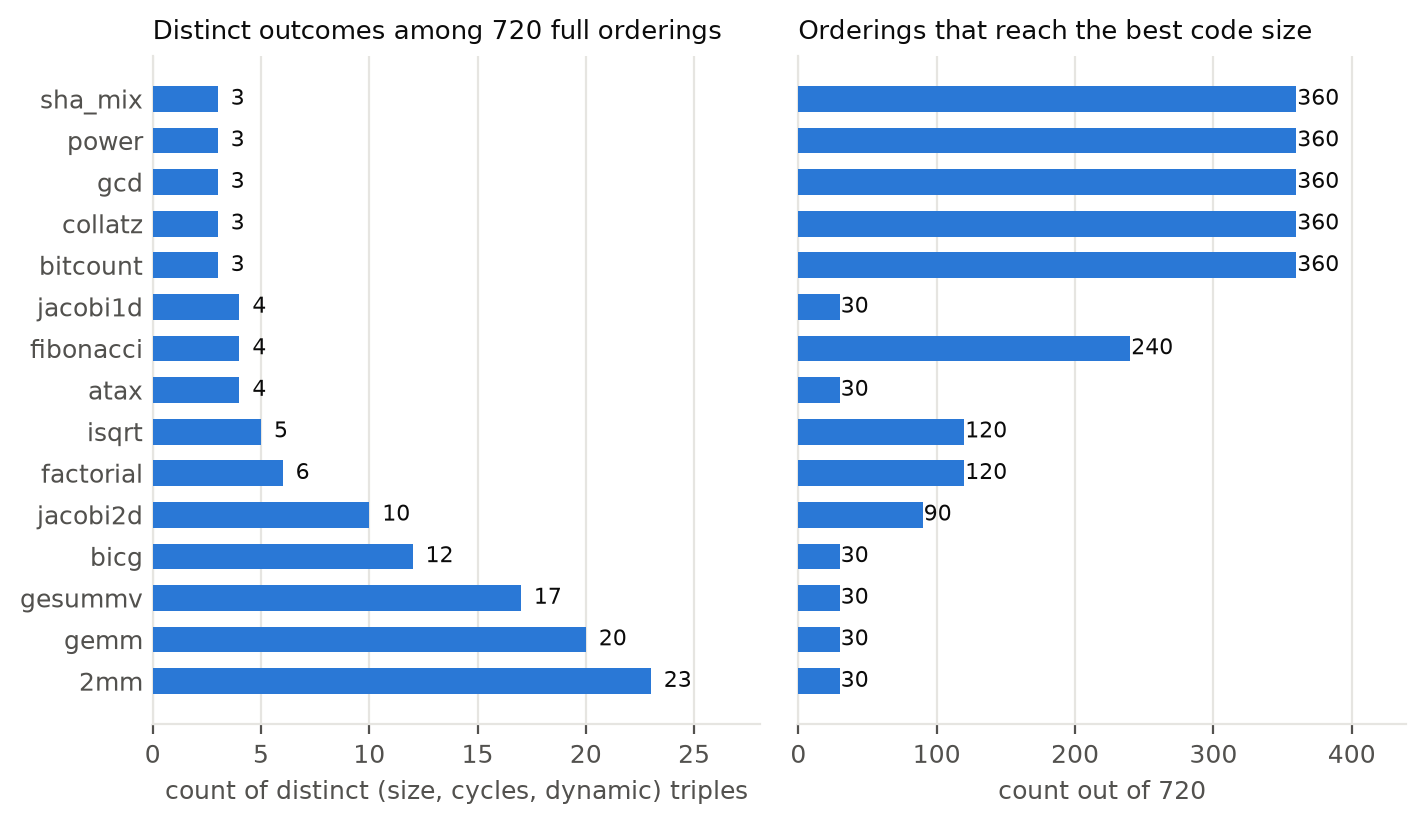
\includegraphics[width=\textwidth]{fig_distinct_outcomes}
\caption[Redundancy of the ordering space per program.]{Redundancy of the ordering space. Left: the number of distinct outcomes among the 720 full orderings; right: the number of orderings that reach the best code size. For the six most array-intensive kernels only one relative order of the four size-relevant passes, 30 orderings, reaches the optimum; for the simplest scalar kernels half of all orderings do.}
\label{fig:distinct}
\end{figure}

The right-hand panel exposes a practical consequence. On the simple scalar programs, 360 of 720 orderings, every ordering in which DCE follows both CF and CP, reach the best size; a compiler writer choosing an order by intuition would have an even chance of being optimal. On the six most array-intensive kernels, only 30 orderings, exactly the class-1 relative order, reach the optimum, and a randomly chosen ordering has a one-in-24 chance. The harder the program, the more precisely the passes must be sequenced.

\fig{fig:position} quantifies the same structure as a marginal effect: the mean normalized code size over all orderings in which a given pass runs first, against those in which it runs last. Moving DCE from first to last improves the mean ratio from 0.988 to 0.659; moving CP from last to first improves it from 0.873 to 0.681; CF from 0.841 to 0.707. CSE's position barely matters (0.789 against 0.793), and SR and AS have no effect at all.


\begin{figure}[!htb]
\centering
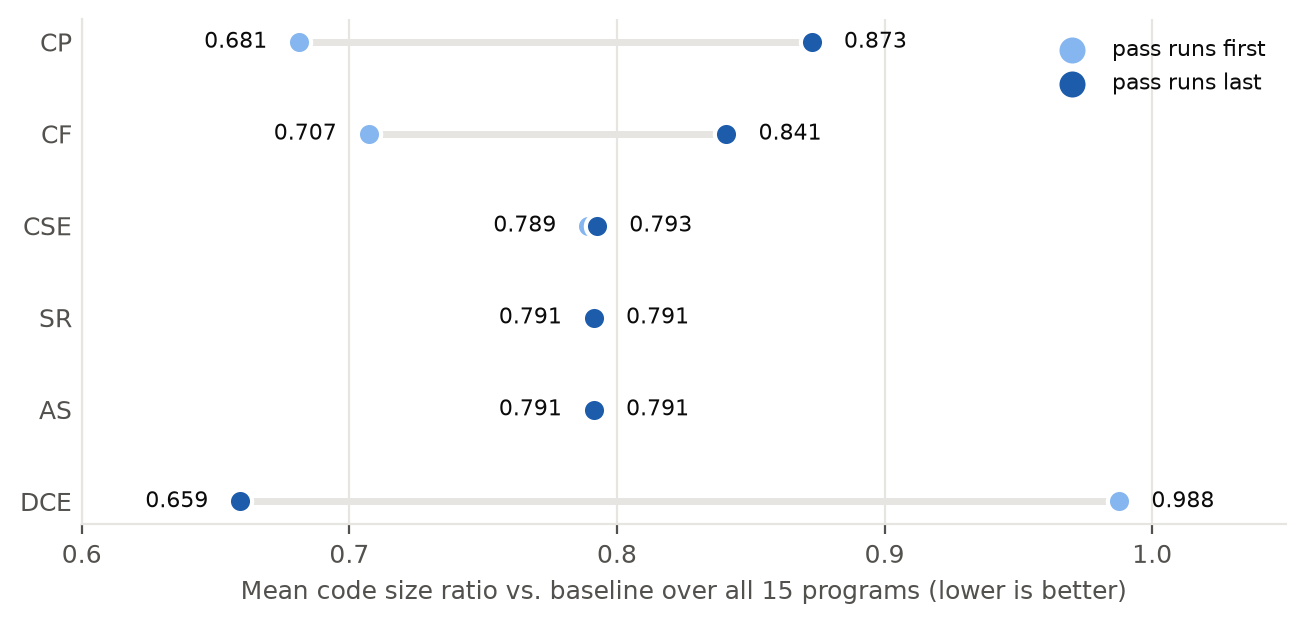
\includegraphics[width=0.92\textwidth]{fig_position_effect}
\caption[Marginal effect of each pass's position on code size.]{Marginal effect of each pass's position. Each row compares the mean normalized code size of the 120 orderings in which the pass runs first (light) with the 120 in which it runs last (dark). DCE is the only pass that should run late; CF and CP should run early; SR and AS do not affect size.}
\label{fig:position}
\end{figure}

\subsubsection*{Pairwise pass interactions}

Table~\ref{tab:interaction} shows the pairwise interaction matrix for \code{gemm}, computed by the visualizer as the mean code size of orderings with pass $A$ before pass $B$ minus that of orderings with $B$ before $A$; \fig{fig:interaction-heatmap} is the corresponding heatmap. A negative entry means $A$ should precede $B$.

\begin{table}[!htb]
\centering\small
\caption{Pairwise interaction matrix for \code{gemm}: mean code size with row pass before column pass minus the reverse (instructions)}
\label{tab:interaction}
\begin{tabular}{L{1.6cm} C{1.4cm} C{1.4cm} C{1.4cm} C{1.4cm} C{1.4cm} C{1.4cm}}
\toprule
\textbf{A $\downarrow$ before B $\rightarrow$} & \textbf{AS} & \textbf{CF} & \textbf{CP} & \textbf{CSE} & \textbf{DCE} & \textbf{SR}\\
\midrule
AS  & 0 & $+$8.1 & $+$6.0 & $+$0.4 & $-$14.4 & 0\\
CF  & $-$8.1 & 0 & $-$2.1 & $-$7.8 & $-$30.4 & $-$8.1\\
CP  & $-$6.0 & $+$2.1 & 0 & $-$5.3 & $-$26.8 & $-$6.0\\
CSE & $-$0.4 & $+$7.8 & $+$5.3 & 0 & $-$14.8 & $-$0.4\\
DCE & $+$14.4 & $+$30.4 & $+$26.8 & $+$14.8 & 0 & $+$14.4\\
SR  & 0 & $+$8.1 & $+$6.0 & $+$0.4 & $-$14.4 & 0\\
\bottomrule
\end{tabular}
\end{table}

\begin{figure}[!htb]
\centering
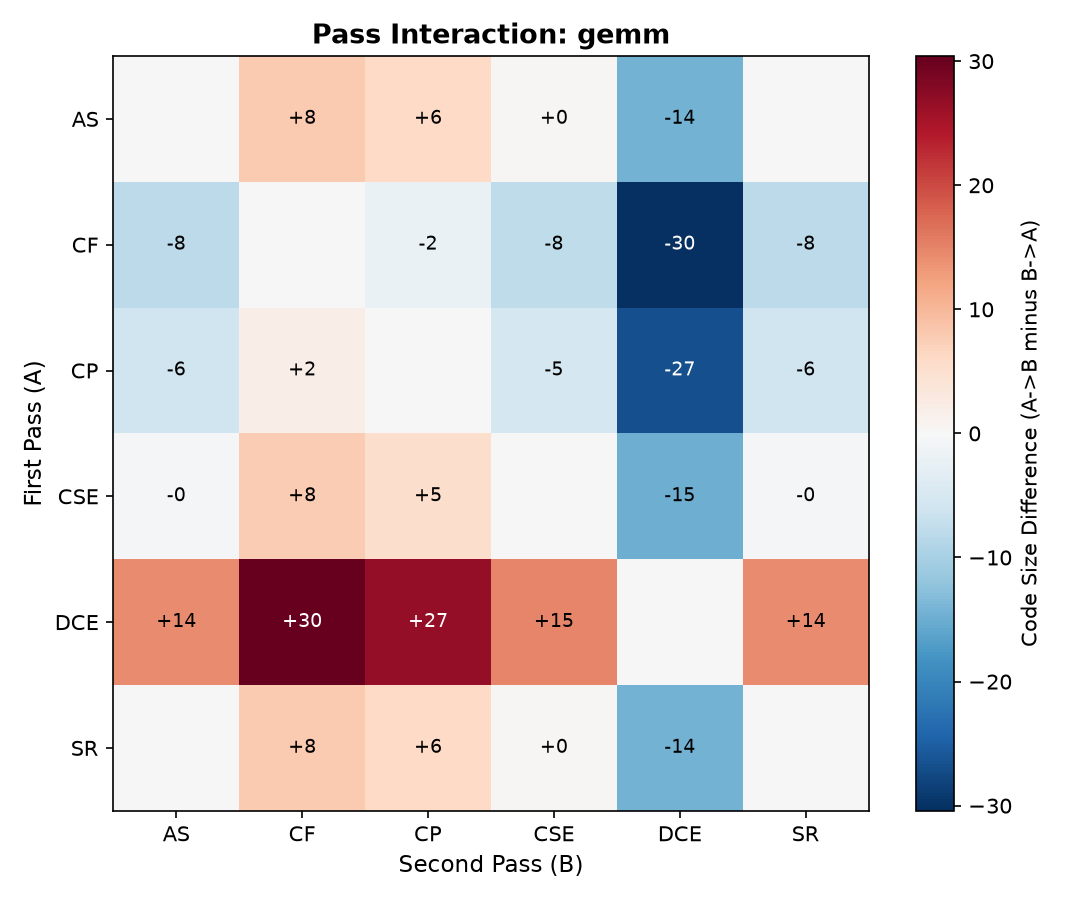
\includegraphics[width=0.55\textwidth]{gemm_pass_interaction}
\caption[Pass interaction heatmap for \code{gemm}.]{Pass interaction heatmap for \code{gemm} produced by the visualizer. Blue cells (negative) indicate that the row pass should run before the column pass; the CF and CP rows against the DCE column carry the largest effects.}
\label{fig:interaction-heatmap}
\end{figure}

The matrix confirms the rules with the direction and magnitude of each pair. Placing CF before DCE saves 30 instructions on average out of 164; CP before DCE saves 27; CSE before DCE saves 15; CF before CP saves 2. The matrix also illustrates a subtlety of marginal analysis. The AS and SR rows are identical and non-zero, even though neither pass ever changes the instruction count. Their entries are not causal: because the matrix averages over all orderings, ``AS before CF'' is correlated with ``DCE relatively later'' in the population of orderings, and the entry reflects the DCE effect rather than any effect of AS. The equivalence-class analysis above, which controls for the other passes, is the correct tool for attribution; the marginal matrix is the right tool for a quick view of which pairs matter most.

\subsubsection*{Where the reduction happens}

\fig{fig:stage-trace} follows the code size of \code{factorial} through each stage of three orderings. Under the best ordering the size stays at 40 through CF, CSE, and CP and drops to 16 at DCE. The enabling passes do not remove a single instruction; they replace instructions with equivalents (a folded expression becomes a LOAD\_CONST, a recomputation becomes a COPY, an operand is renamed) that leave other instructions unread. All of the visible reduction is booked by DCE, but almost none of it is DCE's own doing: run first, DCE removes only the seven planted dead instructions and the ordering ends at 33. Running DCE in the middle, after CF but before CSE and CP, ends at 21. The stage view makes the enabling and consuming roles of the passes visible in a way that final numbers alone cannot; the Optimization Lab page presents exactly this view for any program and ordering.

\begin{figure}[!htb]
\centering
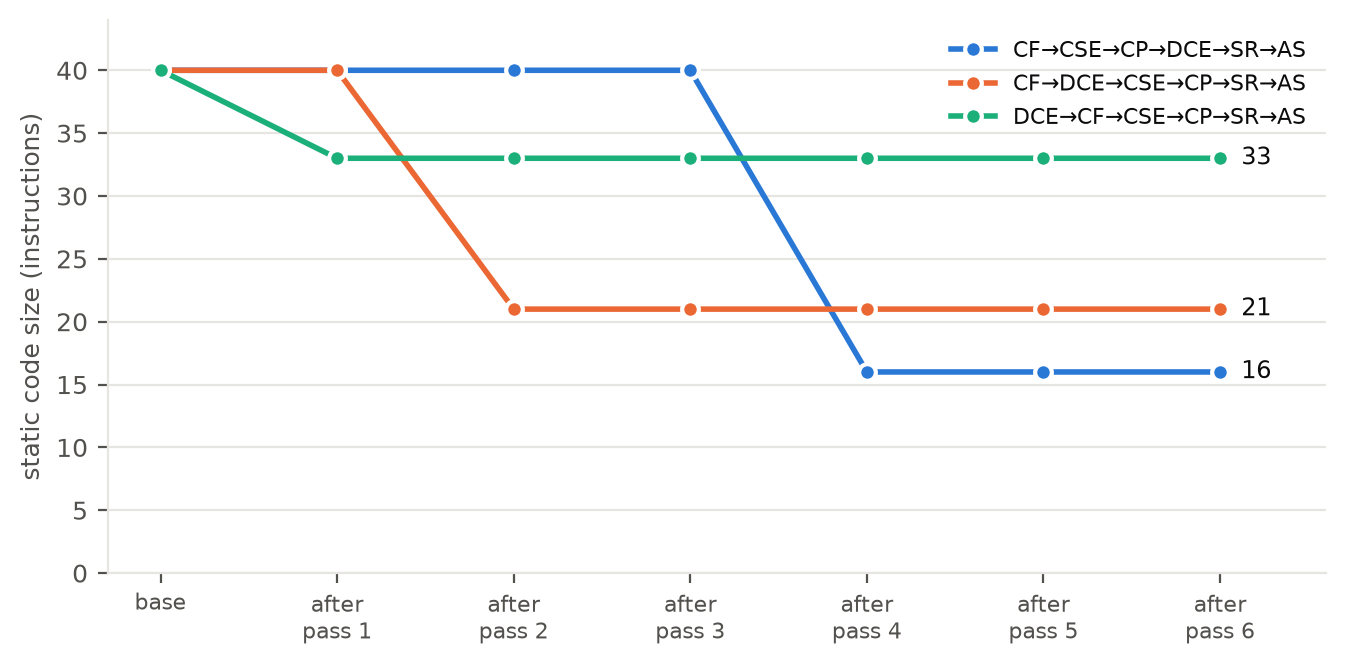
\includegraphics[width=0.9\textwidth]{fig_stage_trace_factorial}
\caption[Code size after each stage of three orderings on \code{factorial}.]{Code size of \code{factorial} after each stage of three orderings. Under the best ordering nothing shrinks until DCE runs; under a DCE-first ordering, DCE removes only the planted dead code and the enabling passes that follow find no consumer for what they expose.}
\label{fig:stage-trace}
\end{figure}

\subsubsection*{Trade-off between code size and estimated cycles}

\fig{fig:pareto} plots every distinct outcome for \code{gemm} in the size-against-cycles plane with the Pareto front drawn by the visualizer. Across all fifteen programs, the two metrics are strongly correlated across orderings: the class with the smallest code is also the class with the lowest cycle estimate and the lowest dynamic count, so in this study there is no trade-off to resolve at the level of classes. There is a residual trade-off within a class, visible as the cycle range in Table~\ref{tab:classes}. It is caused by strength reduction: SR rewrites \code{x * 2} as \code{x + x} (three cycles to one) only when the literal 2 is written in the instruction, and after IR generation the literal sits in a temporary (\code{t4 = 2; t5 = x * t4}). Only constant folding puts the literal into the multiplication, so SR must run after CF to see it. In class 1, orderings with SR after CF have a geometric-mean cycle ratio of 0.7950 and orderings with SR before CF have 0.7999. The Pareto front on \code{gemm} therefore contains points that differ only in cycles, and the front is short: the single best point dominates every other class.

\begin{figure}[!htb]
\centering
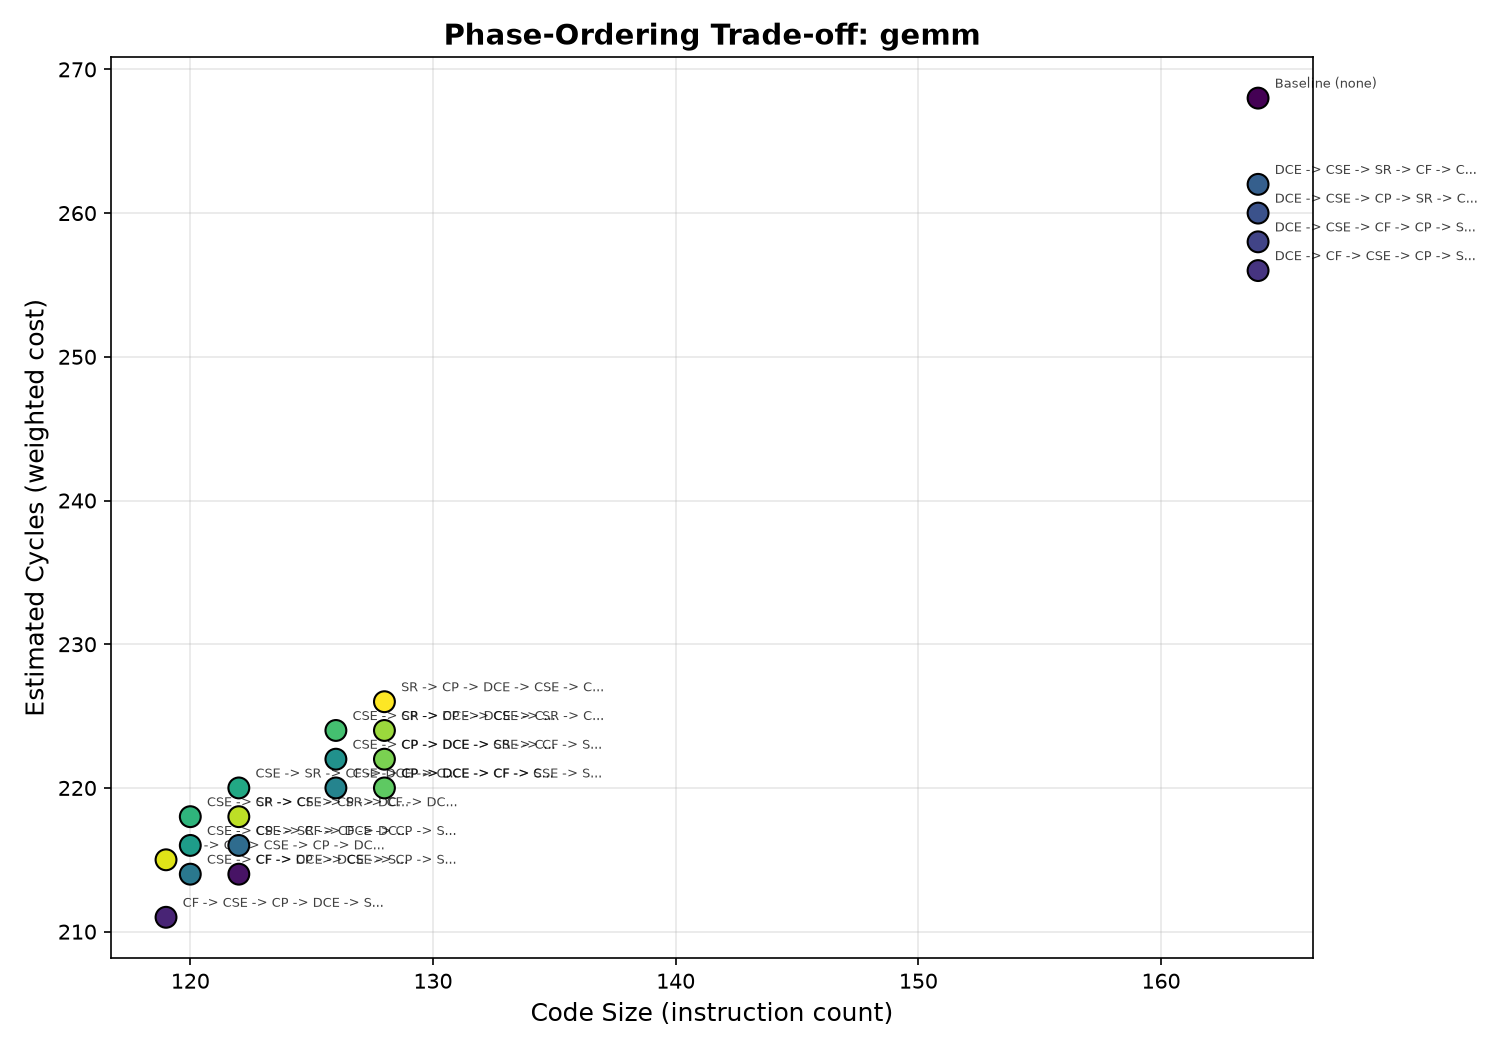
\includegraphics[width=0.78\textwidth]{gemm_tradeoff_scatter}
\caption[Size against estimated cycles for every distinct outcome on \code{gemm}.]{Static code size against estimated cycles for every distinct outcome of the 721 orderings on \code{gemm}, with the Pareto front. Twenty distinct outcomes exist; the best-size class is also the best-cycle class.}
\label{fig:pareto}
\end{figure}


\subsubsection*{Limits of block-local optimization}

The benchmark also quantifies what the block-local passes cannot do. In the optimized \code{factorial} (Appendix~C), the loop body still contains \code{t3 = result * i; result = t3} and \code{t5 = i + 1; i = t5}: the copies into \code{result} and \code{i} survive because both variables are assigned on every iteration, so they fail the single-assignment test for constant propagation, and copy propagation resets at the loop label so it cannot carry \code{t3} into the next iteration's use of \code{result}. A global analysis over a control-flow graph, or an SSA-based representation, would remove these two copies and one comparison temporary in every loop of every benchmark. The array kernels are affected most, since almost all of their instructions live in loop bodies. The measured reductions are therefore a lower bound on what the six transformations could achieve if implemented globally, and the phase-ordering structure found here would need to be re-examined in that setting.

\subsubsection*{Correctness and validation through the RISC-V back end}

Every one of the 10{,}815 optimized programs produced by the exhaustive benchmark printed exactly the same output as its unoptimized baseline, and every one terminated. This is asserted by the benchmark driver and independently by the test suite, which compiles every benchmark under every ordering and compares outputs. It is the strongest available evidence that the six passes are correct in every position, and it is what allows the results above to be interpreted as optimization rather than as accidental deletion.

Table~\ref{tab:asm} carries the size result through code generation. For each benchmark, the baseline IR and the class-1 optimized IR were lowered to RV32IM assembly, and the assembly instructions were counted, excluding labels, directives, and the constant runtime print routine. The reductions in assembly instruction count range from 13.5\% (\code{bicg}) to 50.4\% (\code{factorial}), with a geometric mean of 26.0\% against 35.7\% at the IR level. The assembly reduction is smaller than the IR reduction because the stack-slot back end spends several instructions on every IR instruction that touches memory, and those loads and stores dilute the effect; a register allocator would bring the two figures closer. The test suite verifies that, for all fifteen benchmarks, the assembly produced from the optimized IR prints the same values in the RV32IM simulator as the interpreter produces from the same IR, and returns the same exit status.

\begin{table}[!htb]
\centering\small
\caption{Static size at the IR level and at the RV32IM assembly level, baseline versus best ordering}
\label{tab:asm}
\begin{tabular}{L{1.8cm} C{1.5cm} C{1.5cm} C{1.6cm} C{1.6cm} C{1.6cm} C{1.9cm}}
\toprule
 & \multicolumn{2}{c}{\textbf{IR instructions}} & \multicolumn{3}{c}{\textbf{RV32IM instructions}} & \\
\cmidrule(lr){2-3}\cmidrule(lr){4-6}
\textbf{Program} & base & best & base & best & red.\ \% & \textbf{Simulator}\\
\midrule
2mm & 252 & 185 & 775 & 629 & 18.8 & output matches\\
atax & 101 & 78 & 340 & 292 & 14.1 & output matches\\
bicg & 94 & 73 & 342 & 296 & 13.5 & output matches\\
bitcount & 33 & 19 & 102 & 74 & 27.5 & output matches\\
collatz & 42 & 26 & 123 & 91 & 26.0 & output matches\\
factorial & 40 & 16 & 119 & 59 & 50.4 & output matches\\
fibonacci & 22 & 13 & 61 & 43 & 29.5 & output matches\\
gcd & 21 & 14 & 70 & 56 & 20.0 & output matches\\
gemm & 164 & 119 & 507 & 409 & 19.3 & output matches\\
gesummv & 106 & 78 & 385 & 323 & 16.1 & output matches\\
isqrt & 50 & 27 & 140 & 84 & 40.0 & output matches\\
jacobi1d & 76 & 50 & 254 & 191 & 24.8 & output matches\\
jacobi2d & 144 & 95 & 476 & 346 & 27.3 & output matches\\
power & 71 & 47 & 184 & 136 & 26.1 & output matches\\
sha\_mix & 106 & 68 & 290 & 214 & 26.2 & output matches\\
\midrule
\textbf{Geomean ratio} & & \textbf{0.6426} & & & \textbf{0.7402} & \\
\bottomrule
\end{tabular}
\end{table}

\section{Non Functional Requirements Results Achieved}

All eight non-functional requirements were met. Table~\ref{tab:nfr-status} gives the measured evidence for each.

\begin{table}[!htb]
\centering\small
\caption{Non Functional Requirements Status Table}
\label{tab:nfr-status}
\begin{tabular}{L{1.5cm} L{4.6cm} L{1.6cm} L{5.5cm}}
\toprule
\textbf{NFR} & \textbf{Requirement} & \textbf{Status} & \textbf{Measured result}\\
\midrule
NFR-1 & Correctness under every ordering and after lowering & Achieved & 10{,}815 of 10{,}815 optimized programs match baseline output; 15 of 15 benchmarks match in the RV32IM simulator\\
NFR-2 & Determinism and reproducibility & Achieved & Repeated runs and runs on Linux and Windows produce identical IR, assembly, and metric tables; no randomness in any module\\
NFR-3 & Performance: single-program exhaustive benchmark $<$ 10 s; all programs $<$ 60 s & Achieved & Slowest program (\code{2mm}) 5.21 s; fastest (\code{gcd}) 0.17 s; all fifteen programs with plots 23.5 s\\
NFR-4 & Transparency and readability & Achieved & Compiler core about 4{,}000 lines in 19 modules; largest module 560 lines; every module has an algorithm description at its head\\
NFR-5 & Portability and ease of installation & Achieved & Pure Python 3.10+ with five pip dependencies; pre-built front end committed; no database, network, or CDN dependency; verified on Linux and Windows\\
NFR-6 & Usability & Achieved & Keyboard reordering of passes; errors reported with phase, message, line, and column and underlined in the editor; compile and optimize responses well under one second for all benchmarks\\
NFR-7 & Maintainability and test coverage & Achieved & 185 test cases in 3 modules, all passing in 3.98 s; type annotations throughout; tests run before every merge\\
NFR-8 & Extensibility & Achieved & Adding a pass requires one module and one registry entry; verified when CP, SR, and AS were added after CF, DCE, and CSE with no change to the pass manager, benchmark, or API\\
\bottomrule
\end{tabular}
\end{table}

Two of the requirements deserve comment. NFR-3 was set so that the Phase-Ordering Explorer could run the exhaustive benchmark interactively in the browser; the measured 5.2 seconds for the largest program, most of it spent interpreting 721 optimized programs of 4{,}000 to 5{,}000 executed instructions each, leaves comfortable margin, and programs of the size a student would type run in well under a second. NFR-4 is the requirement that distinguishes this project from a study on a production compiler; the line counts per module reported in Chapter 4 are the evidence that it was met, and the fact that every result in this chapter can be traced by hand through the listings in Appendix~C is its practical consequence.

\section{Comparison of Results with Existing Works}

Direct numerical comparison with the literature is limited by two differences. The published studies use production or research compilers with tens to hundreds of passes, so their orderings and ours are not the same objects; and most of them report improvements over an already-optimized baseline such as \code{-O3} or \code{-Oz}, whereas this project reports improvements over unoptimized code, because the unoptimized IR is the only baseline that is independent of any ordering. The comparison in Table~\ref{tab:comparison} is therefore made on the structural findings, which are comparable, and the magnitudes are reported with their baselines stated.

\begin{table}[!htb]
\centering\small
\caption{Comparison of the findings of this project with existing work}
\label{tab:comparison}
\begin{tabular}{L{3.0cm} L{5.0cm} L{5.4cm}}
\toprule
\textbf{Work} & \textbf{Their finding} & \textbf{This project}\\
\midrule
Cooper et al.\ \cite{cooper1999} & Genetic search over 10 passes finds program-specific sequences that produce smaller code than the fixed default. & Exhaustive search over 6 passes: the best class is the \emph{same} for all 15 programs, so on this pass set a fixed sequence is optimal. Program specificity appears only in how many orderings are optimal (30 to 360 of 720).\\
Kulkarni et al.\ \cite{kulkarni2004,kulkarni2006} & Most phase sequences produce duplicate function instances; dormant phases are common; exhaustive enumeration of distinct instances is feasible. & 720 orderings produce 3 to 23 distinct outcomes per program (0.4\% to 3.2\%); SR and AS are dormant with respect to size on every program; the class structure is fully enumerated.\\
Muchnick \cite{muchnick1997} & Recommends constant folding early and dead code elimination as a late, repeated clean-up. & Quantified: DCE first gives a 1.2\% mean reduction, DCE last gives 34.1\%; CF first 29.3\% versus CF last 15.9\%.\\
Whitfield \& Soffa \cite{whitfield1997} & Transformations have enabling and disabling relationships that depend on the program. & Only enabling relationships were found among these six passes; no pass disables another on any program (no ordering is worse than the baseline).\\
Jain et al.\ \cite{jain2022} & Reinforcement learning improves code size over LLVM \code{-Oz} while holding execution time; size and time can conflict. & Size and both time proxies are minimized by the same class on all 15 programs; the only residual conflict is SR's position relative to CF, worth 0.5\% of cycles.\\
Cummins et al.\ \cite{cummins2023} & A learned model improves LLVM code size by about 3\% over \code{-Oz}. & 35.7\% over \emph{unoptimized} code; not comparable in magnitude, but the same metric (static instruction count) and the same objective.\\
Georgiou et al.\ \cite{georgiou2018} & On Cortex-M targets the default optimization level is often not the best; pass interactions are the cause. & Consistent: on the array kernels only 1 in 24 relative orders is optimal; a default chosen without measurement would be suboptimal 23 times in 24.\\
Click \& Cooper \cite{click1995} & Combining analyses can beat any sequence of separate passes. & The surviving loop-carried copies in every benchmark are exactly the cases a combined or global analysis would remove; identified as future work.\\
\bottomrule
\end{tabular}
\end{table}

The comparison supports three conclusions. First, the qualitative phenomena reported for production compilers, redundancy of the ordering space, dormancy of some passes, and the enabling role of constant propagation, are reproduced exactly, not approximately, on a six-pass infrastructure, which suggests that they are properties of the transformations themselves rather than of any particular compiler. Second, the program-specificity that motivates search and learning methods at production scale does not appear at this scale: with six local passes a single fixed sequence is optimal for every program tested. Program-specific ordering presumably emerges from the interactions of loop and interprocedural transformations that are absent here, and the infrastructure is positioned to test that hypothesis by adding them. Third, the magnitude of the effect, a factor of more than 25 between the best and worst classes in mean code-size reduction, is large enough that the phase-ordering problem deserves the attention it receives in the literature and in the classroom.

\section{Project GUI Snapshots}
\label{sec:gui}

The interactive application is the delivery vehicle for everything in this chapter. It is served by a single Python process and opens to the Playground. Its design uses a dark, editor-like theme with a monospaced face for code and a sans-serif face for controls, a persistent left sidebar for the five sections, and a ``pipeline rail'' at the top of every page that shows which compiler stages the page exercises. All interactions are available from the keyboard. The fifth section, Reference, documents the passes, the cost model, and the language so that the application is self-contained; the four working sections are shown below.

\subsubsection*{1. Playground}

The Playground (\fig{fig:gui-playground}) is the entry point. The user writes a program in the CodeMirror editor or loads one of the fifteen benchmarks from the example picker, which groups them by suite and shows each program's documentation comment as a title with bullet points. Compiling (button or Ctrl+Enter) fills the right-hand panel, whose tabs show the token stream as coloured chips, the syntax tree as a collapsible outline, the symbol table with scope depths and IR names, and the three-address code. When compilation fails, the badge next to the button names the phase and line, and the editor underlines the offending position; \fig{fig:gui-error} shows a semantic error reported for an undeclared variable.

\begin{figure}[!htb]
\centering
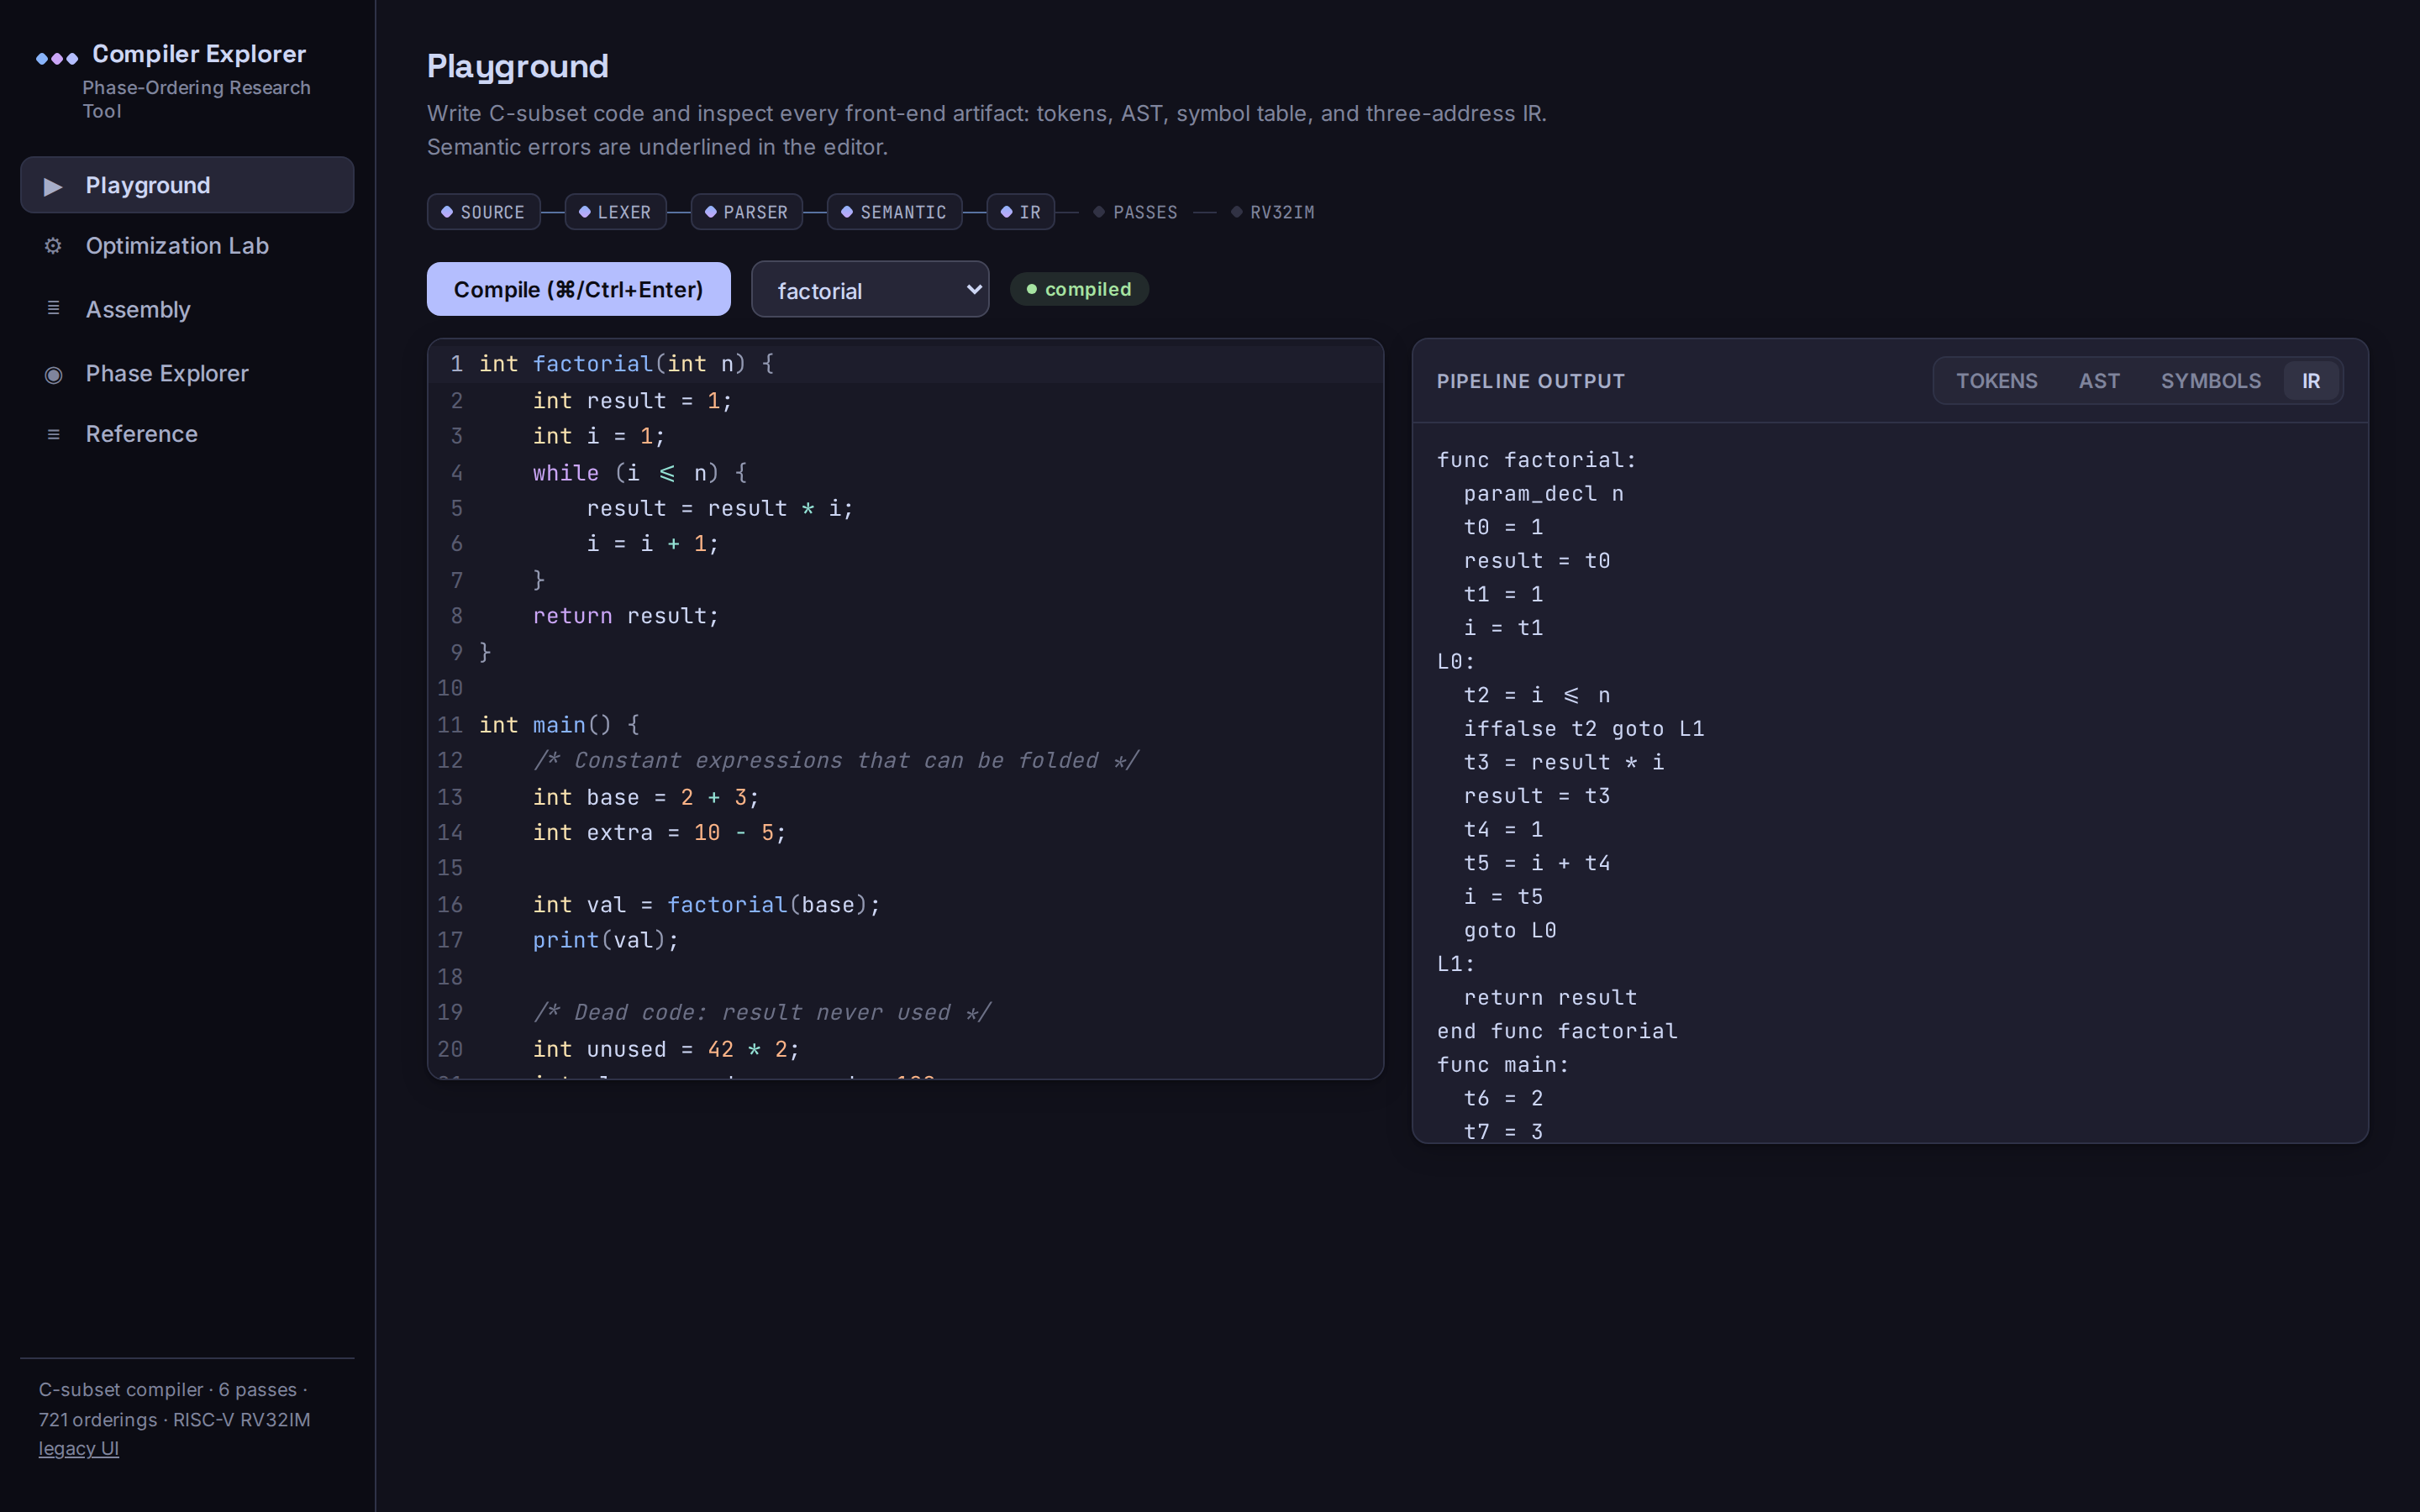
\includegraphics[width=0.82\textwidth]{gui_playground}
\caption[Playground page showing the IR of \code{factorial}.]{Playground page with the \code{factorial} benchmark loaded and compiled; the IR tab shows the three-address code with functions, labels, and temporaries.}
\label{fig:gui-playground}
\end{figure}

\begin{figure}[!htb]
\centering
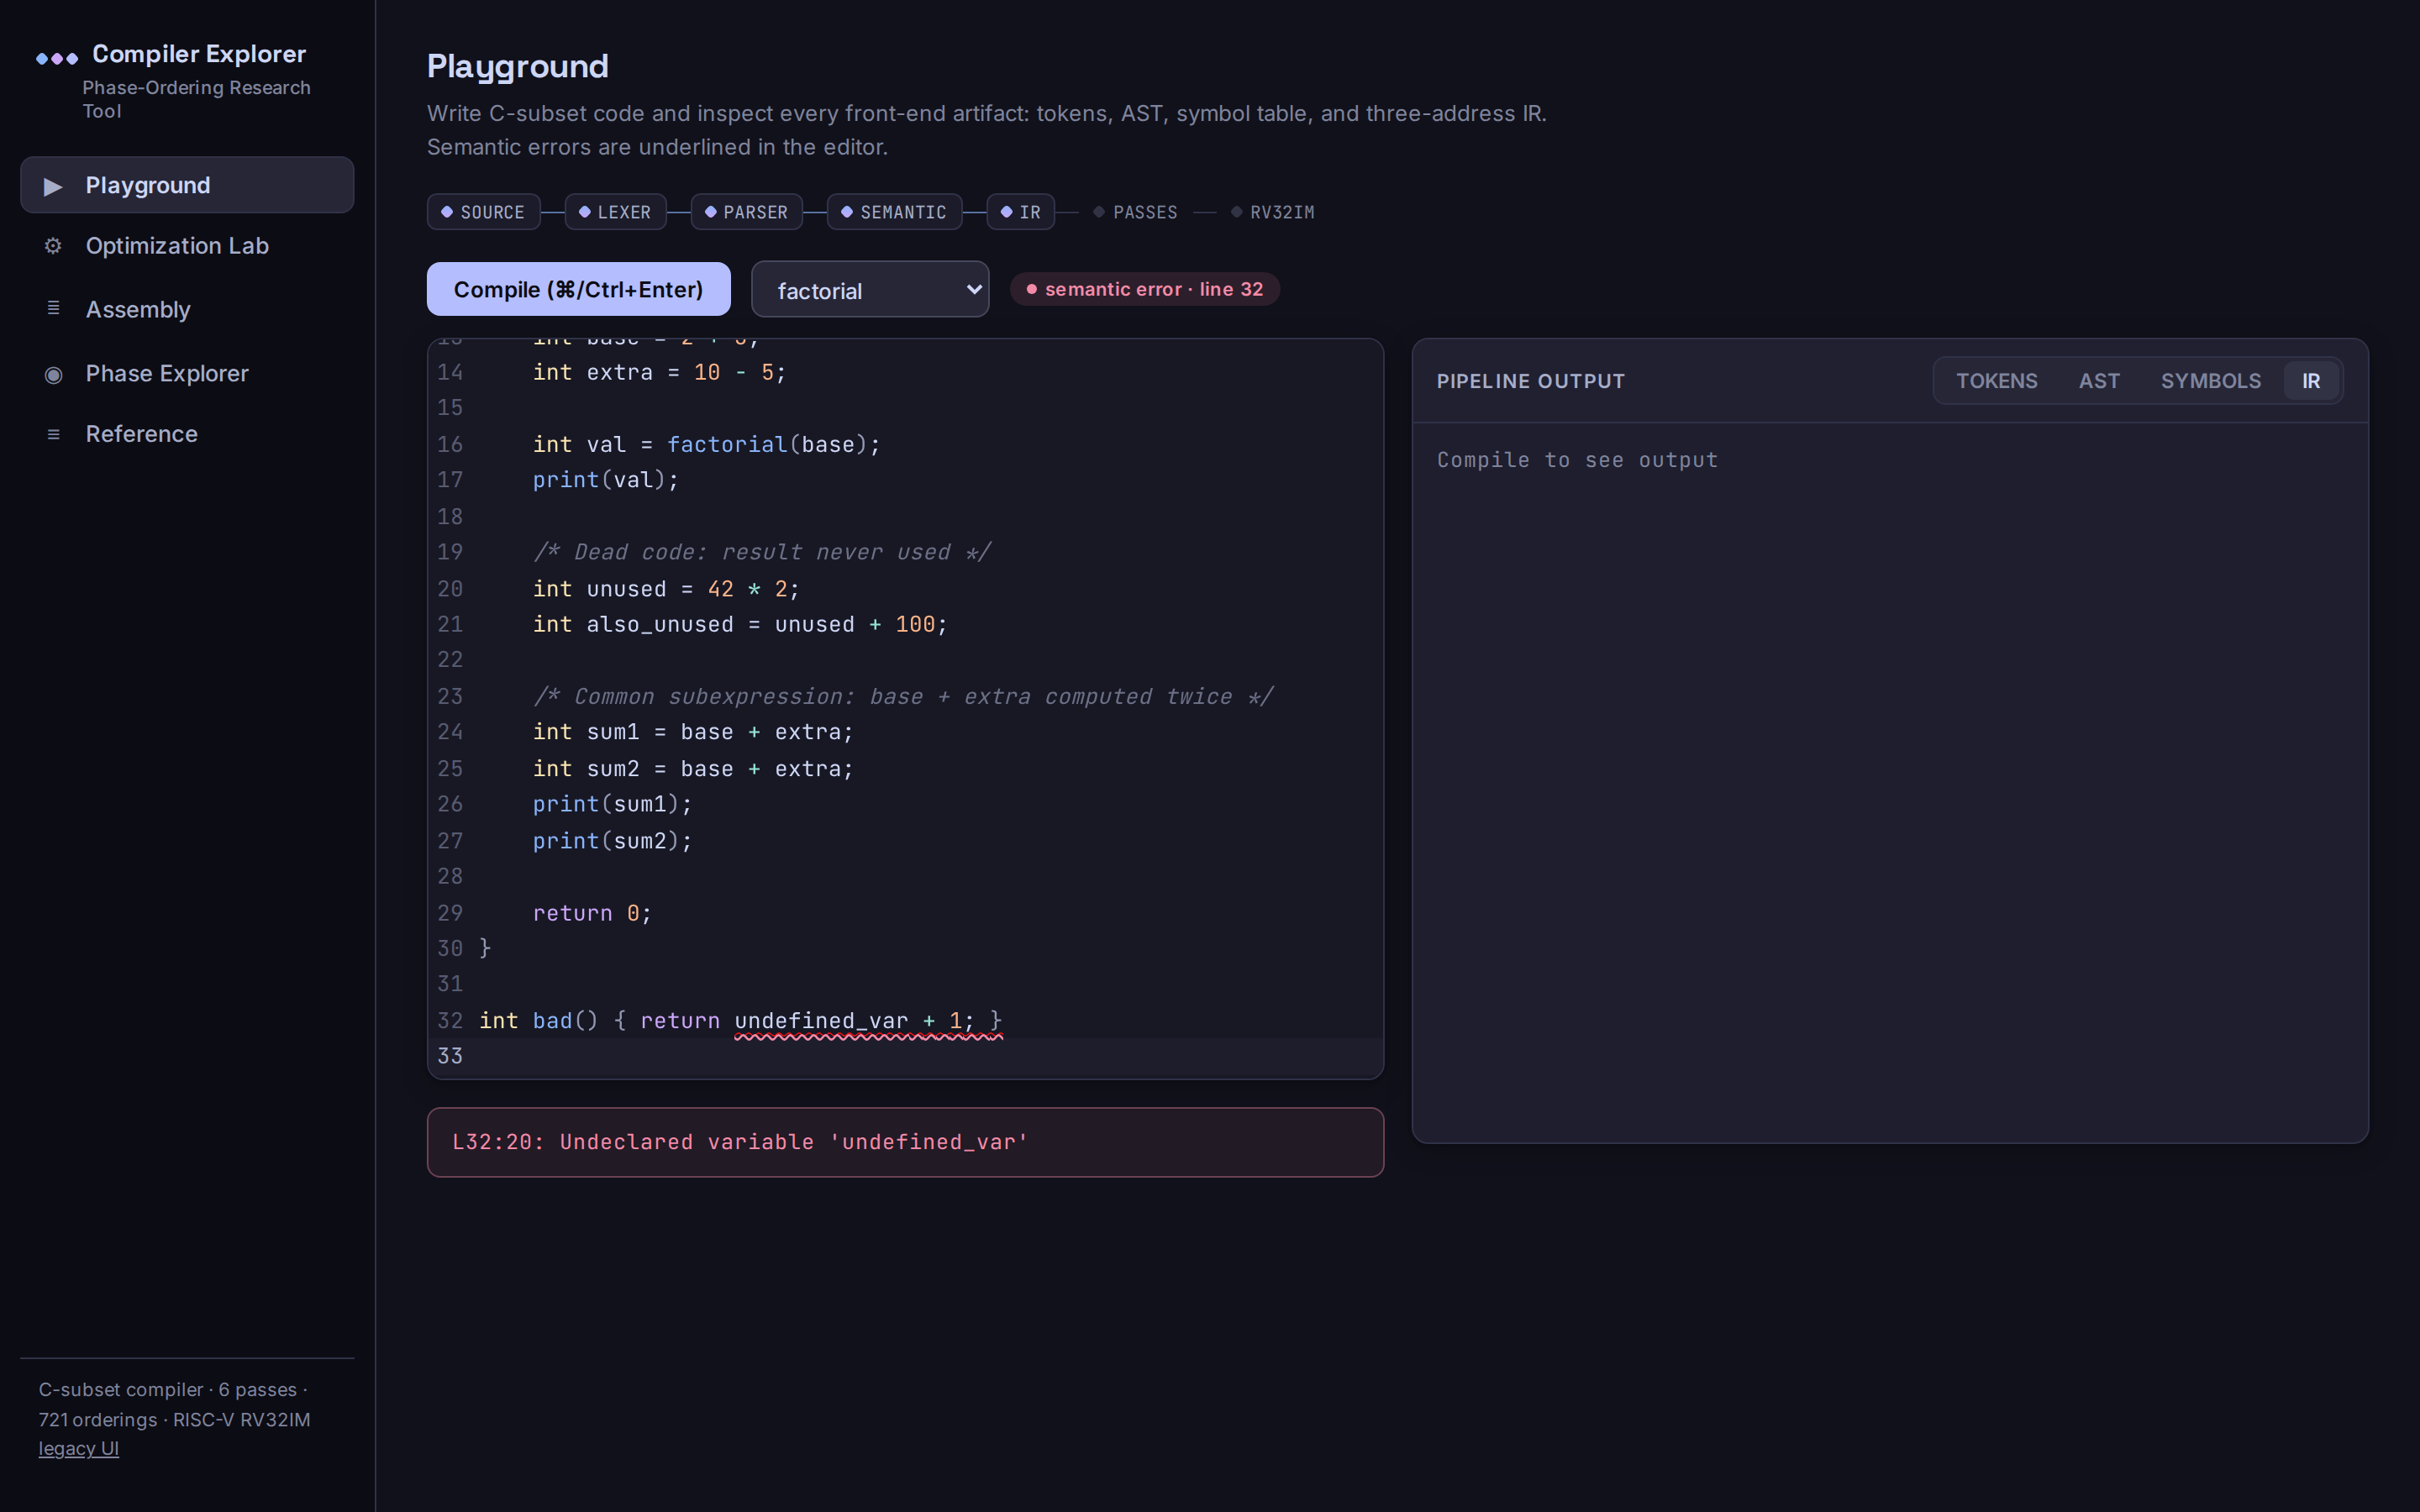
\includegraphics[width=0.82\textwidth]{gui_playground_error}
\caption[Playground page reporting a semantic error.]{Playground page reporting a semantic error. The badge names the phase and line, and the editor underlines the undeclared variable at the reported position.}
\label{fig:gui-error}
\end{figure}

\subsubsection*{2. Optimization Lab}

The Optimization Lab (\fig{fig:gui-optlab}) is the phase-ordering problem made interactive. The six passes appear as numbered chips that can be dragged into any order, or moved with the arrow keys. Running the pipeline produces one card per stage showing the code size after that stage and its delta; selecting a card displays the IR after that stage with lines removed by the pass struck through and lines added highlighted, and the three stat tiles report code size, estimated cycles, and the effect of the selected pass. In the figure, \code{factorial} has been run under the best ordering and the DCE stage is selected, showing the 24 instructions it removed and the strikethrough of the constant-holding temporaries that CF and CP made dead.

\begin{figure}[!htb]
\centering
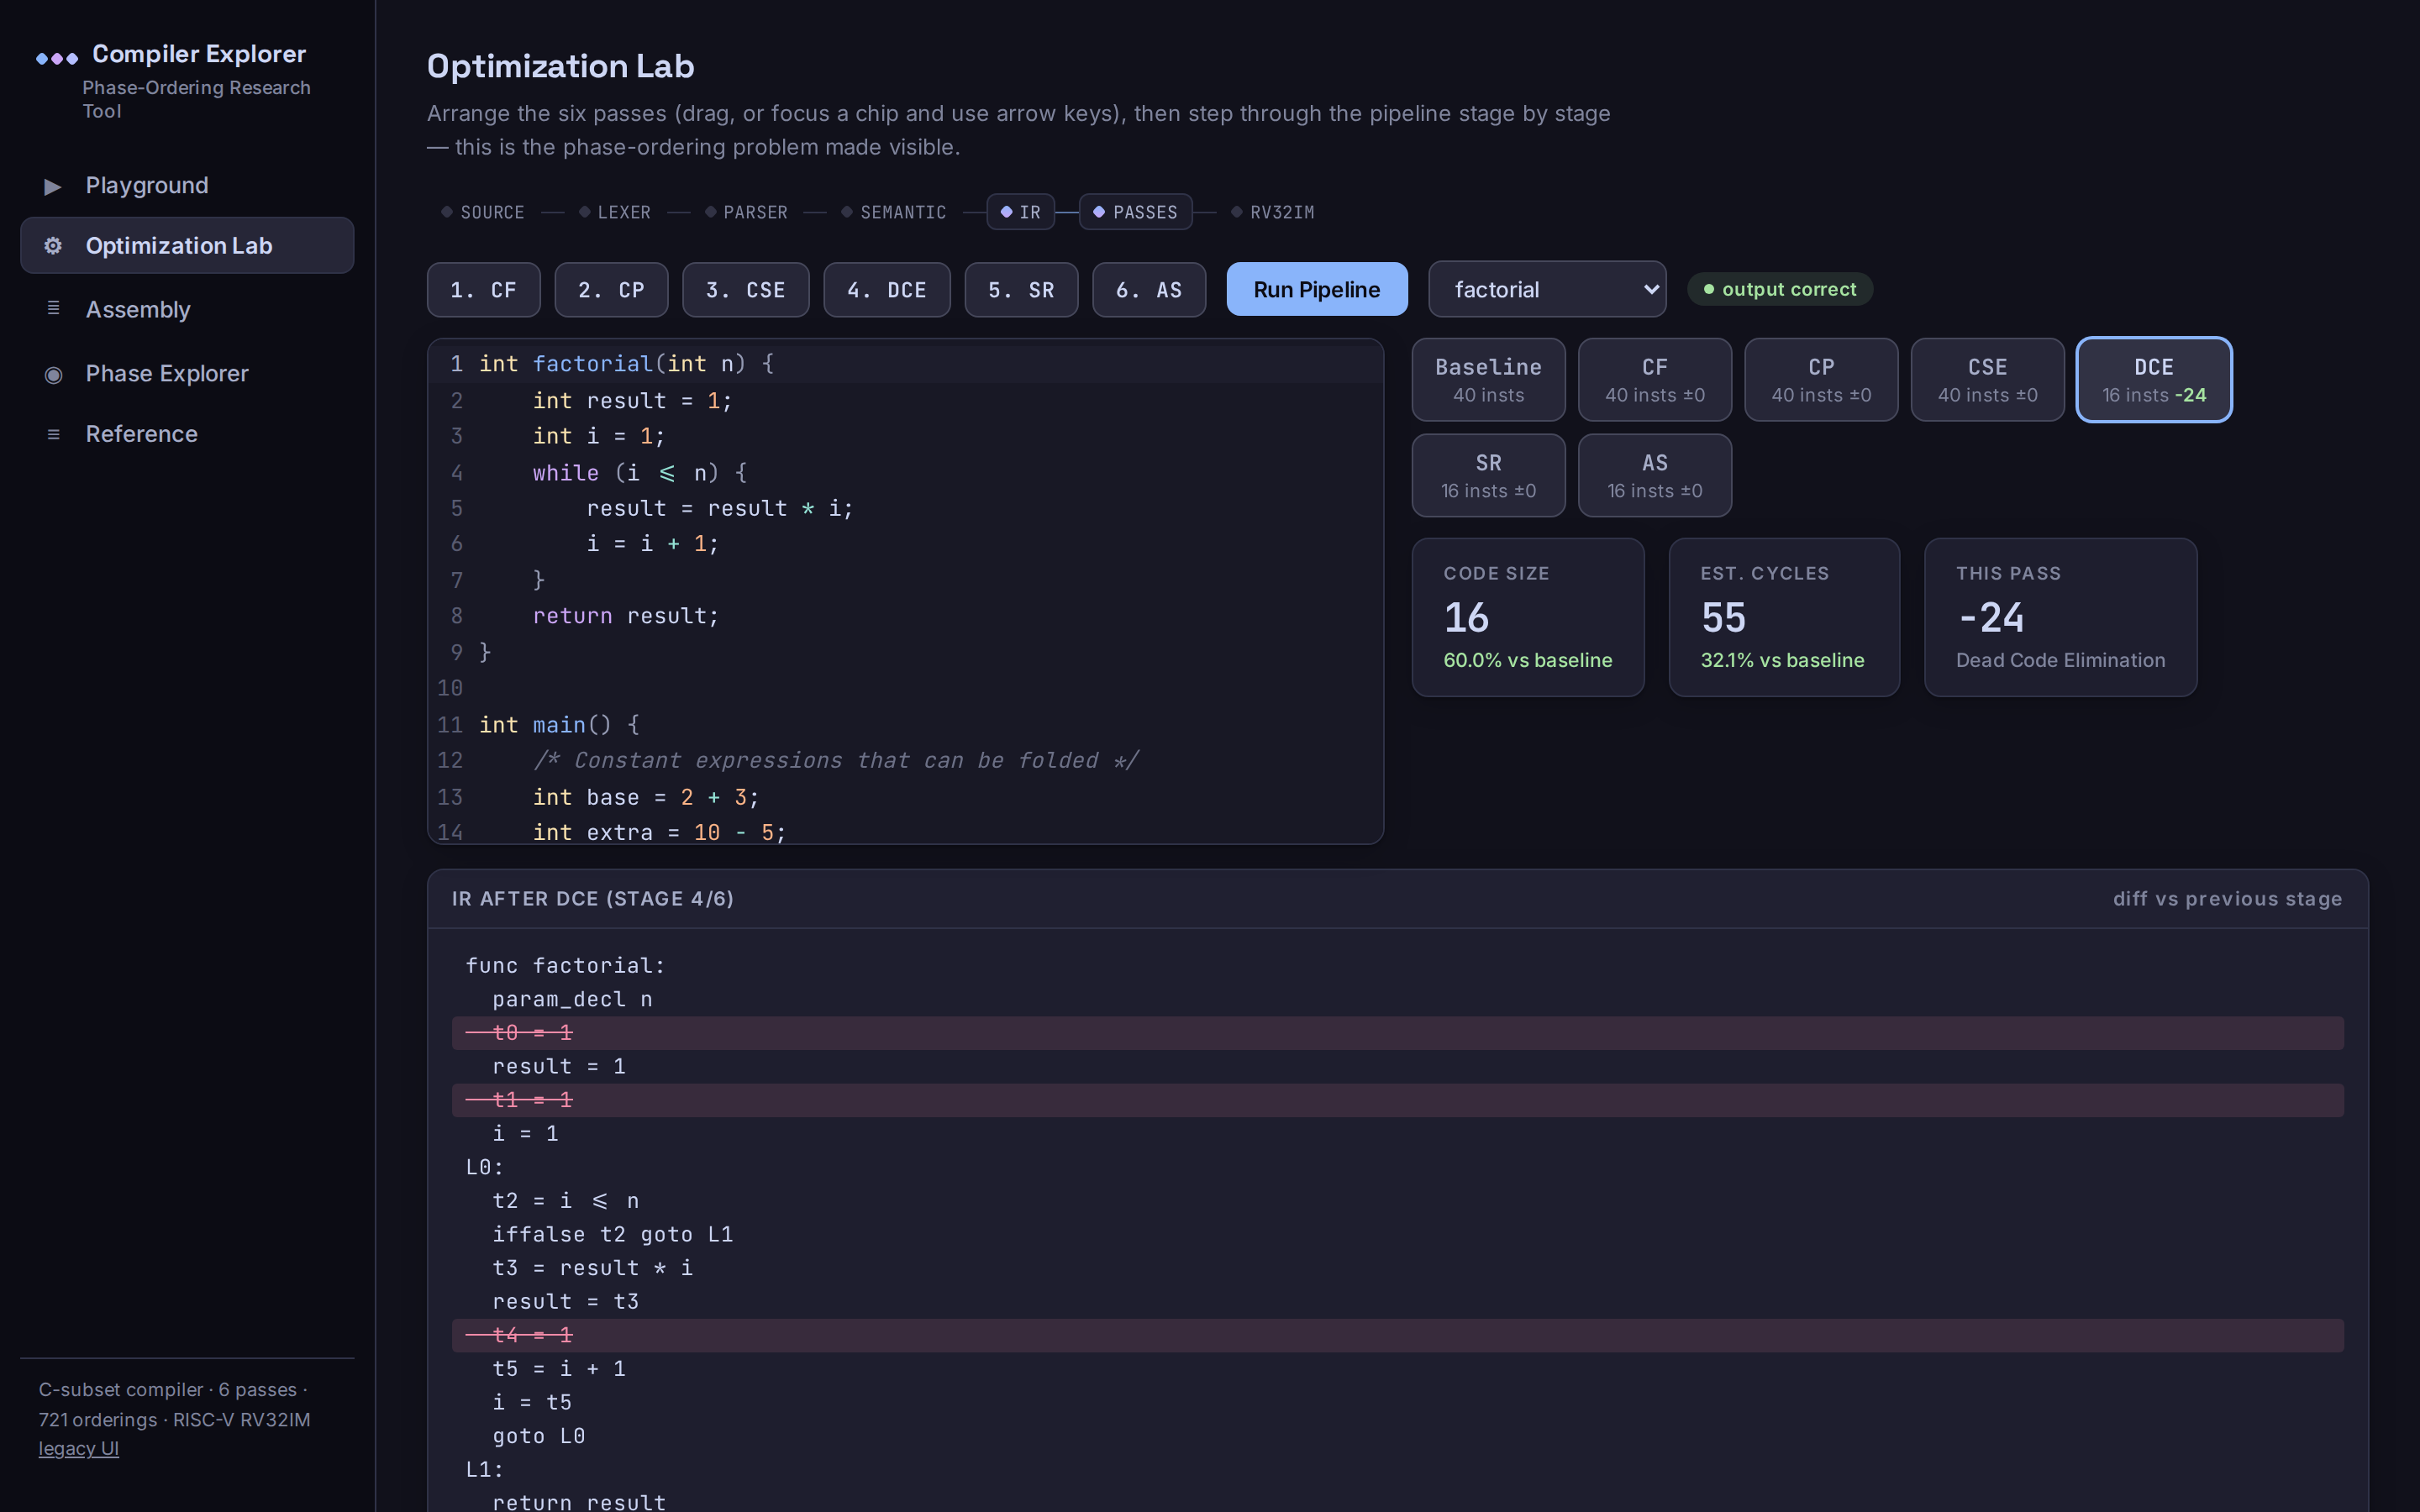
\includegraphics[width=0.82\textwidth]{gui_optlab_diff}
\caption[Optimization Lab page with the DCE stage of the best ordering selected.]{Optimization Lab page: \code{factorial} under CF, CP, CSE, DCE, SR, AS with the DCE stage selected. The stage cards show that no instruction is removed until DCE; the diff view strikes through the 24 instructions DCE removed.}
\label{fig:gui-optlab}
\end{figure}

\subsubsection*{3. Assembly}

The Assembly page (\fig{fig:gui-assembly}) shows the three-address code and the generated RV32IM assembly side by side, with a toggle for optimized or unoptimized input. Hovering over an IR line highlights the assembly lines it produced, using the mapping returned by the assembly endpoint, so that a student can see, for example, that a single \code{t2 = i <= n} becomes two loads, a \code{slt}, an \code{xori}, and a store.

\begin{figure}[!htb]
\centering
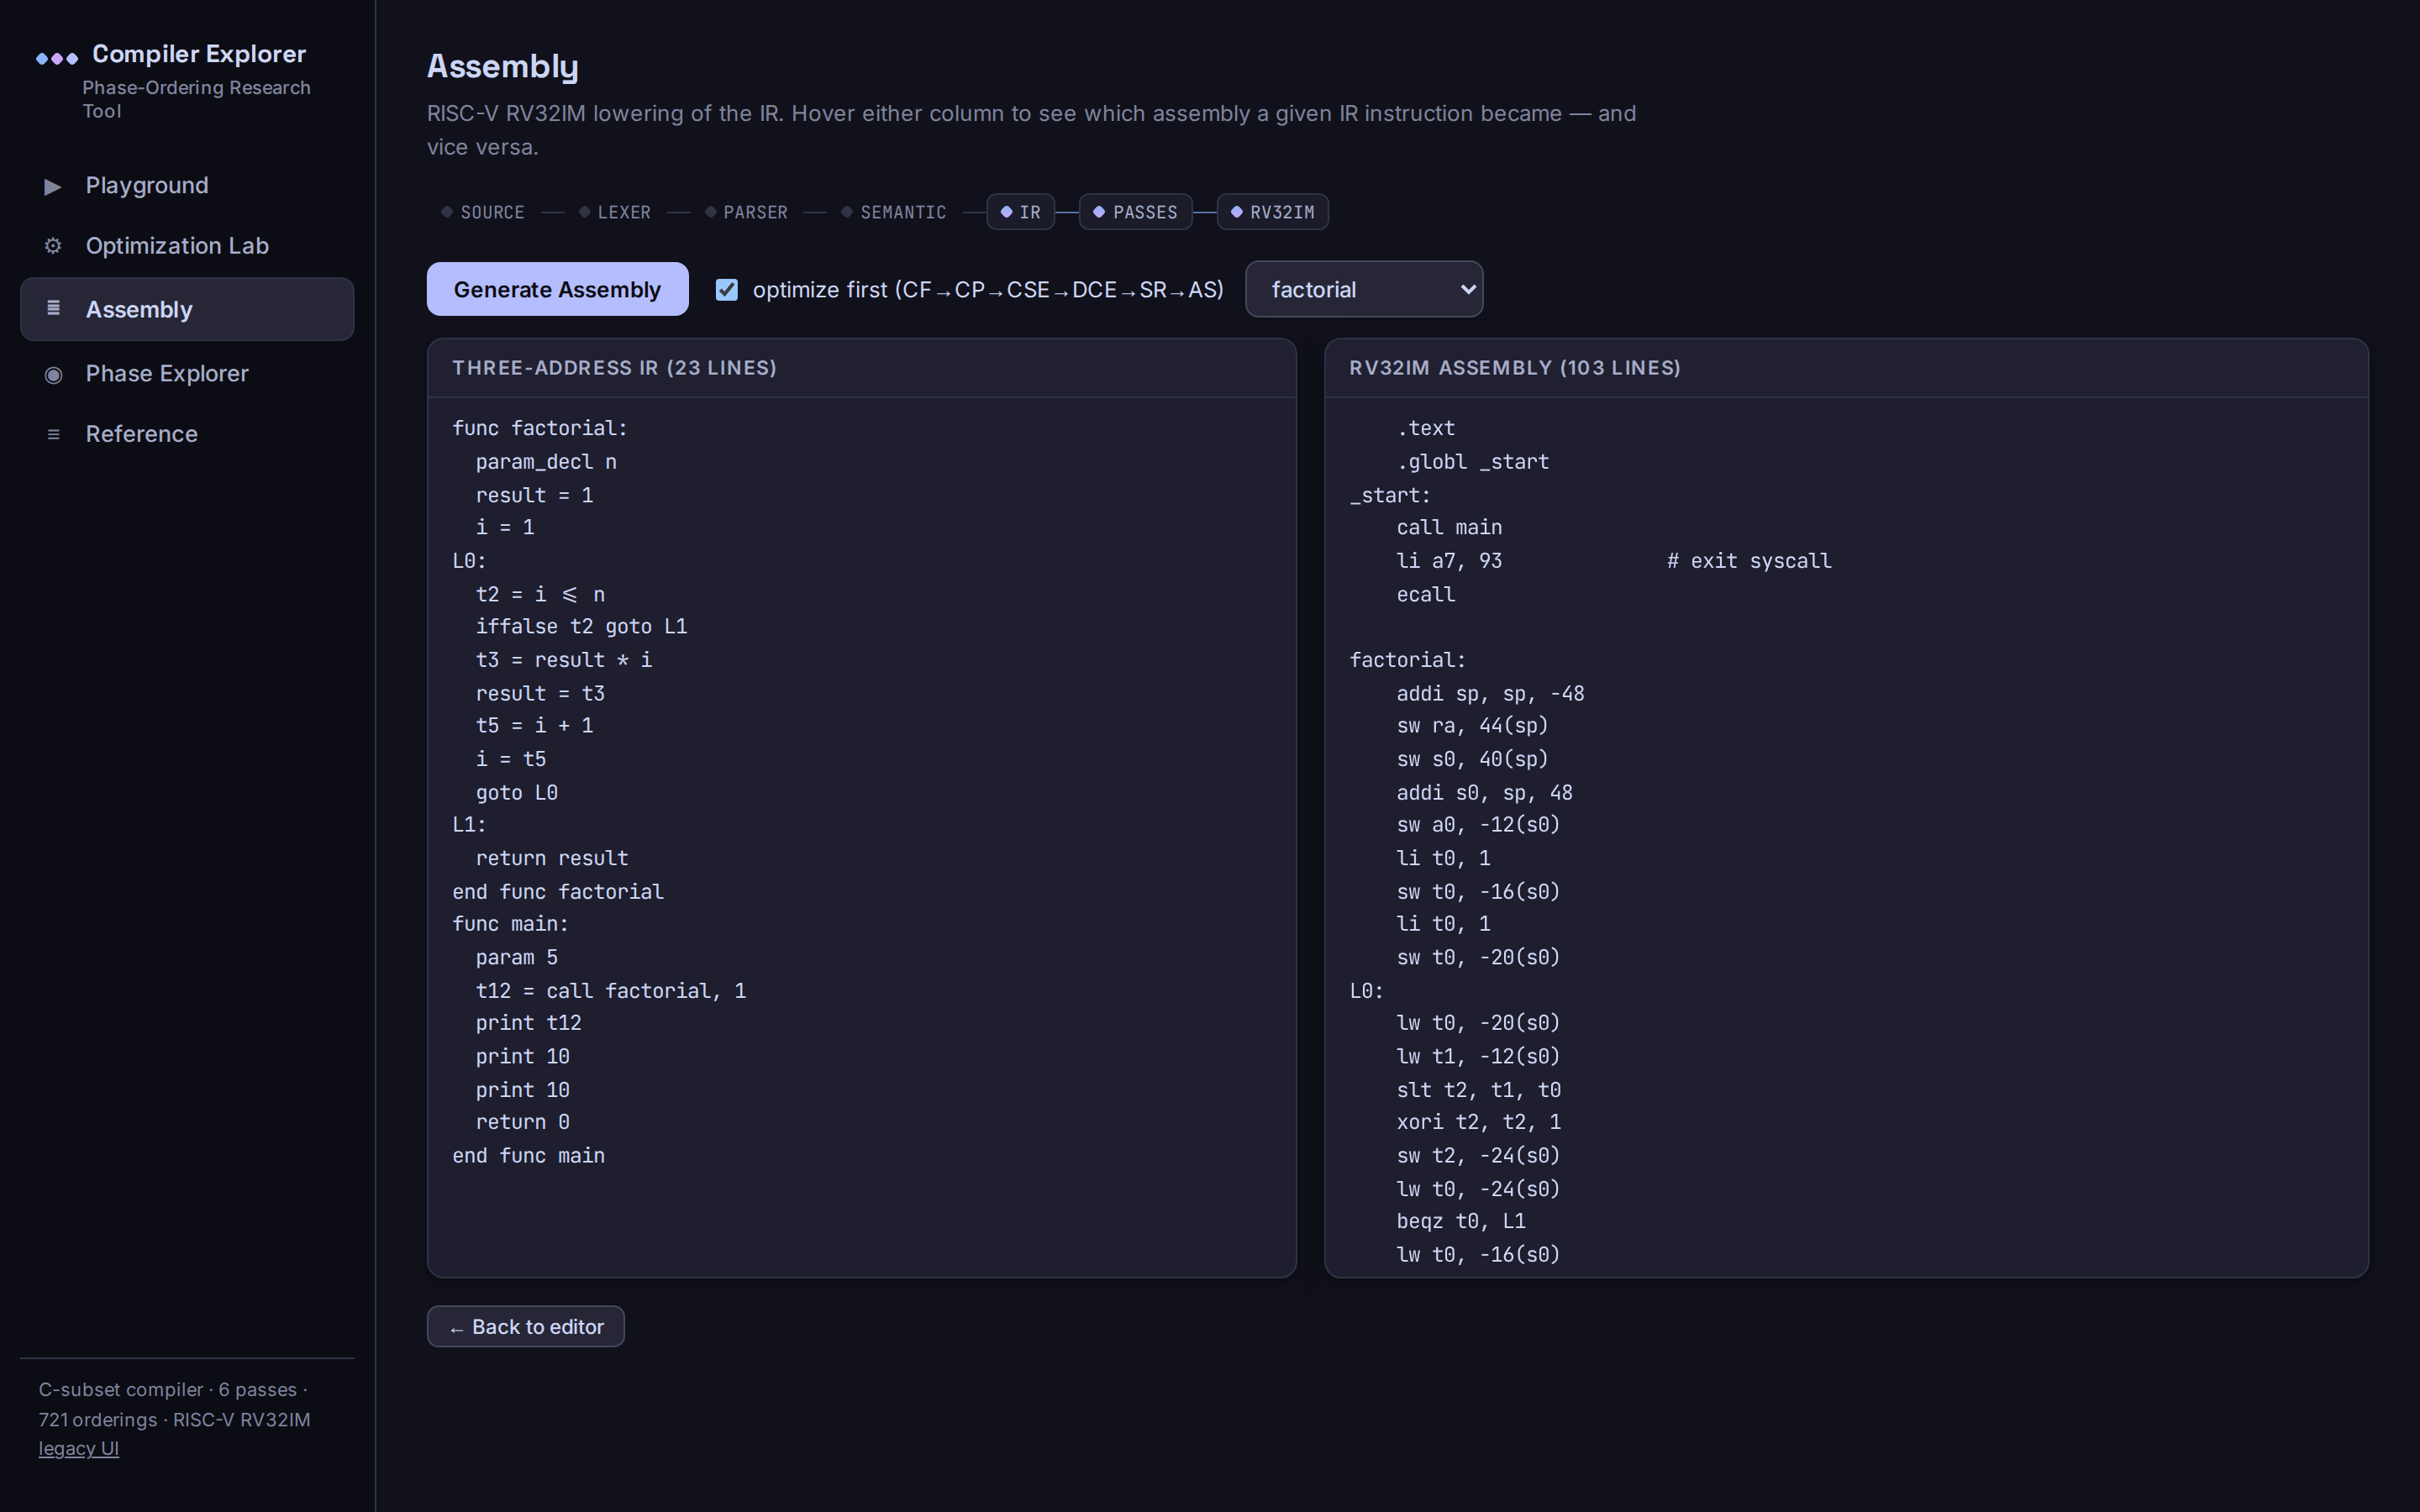
\includegraphics[width=0.82\textwidth]{gui_assembly}
\caption[Assembly page with hover-linked IR and RV32IM assembly.]{Assembly page for \code{factorial}: optimized IR on the left, RV32IM assembly on the right, with hover linking between corresponding lines.}
\label{fig:gui-assembly}
\end{figure}

\subsubsection*{4. Phase-Ordering Explorer}

The Phase-Ordering Explorer (\fig{fig:gui-explorer}) runs all 721 orderings on the current program in the server and plots the results in the browser: a scatter of static code size against estimated cycles with the Pareto-optimal orderings highlighted, and a bar chart of the ten smallest results. Clicking a point reveals its ordering and metrics. The badges report how many orderings are Pareto-optimal and confirm that every ordering's output was verified against the baseline. In the figure, \code{gemm} shows twenty distinct outcomes spread from 119 to 164 instructions, with the best class at the lower left.

\begin{figure}[!htb]
\centering
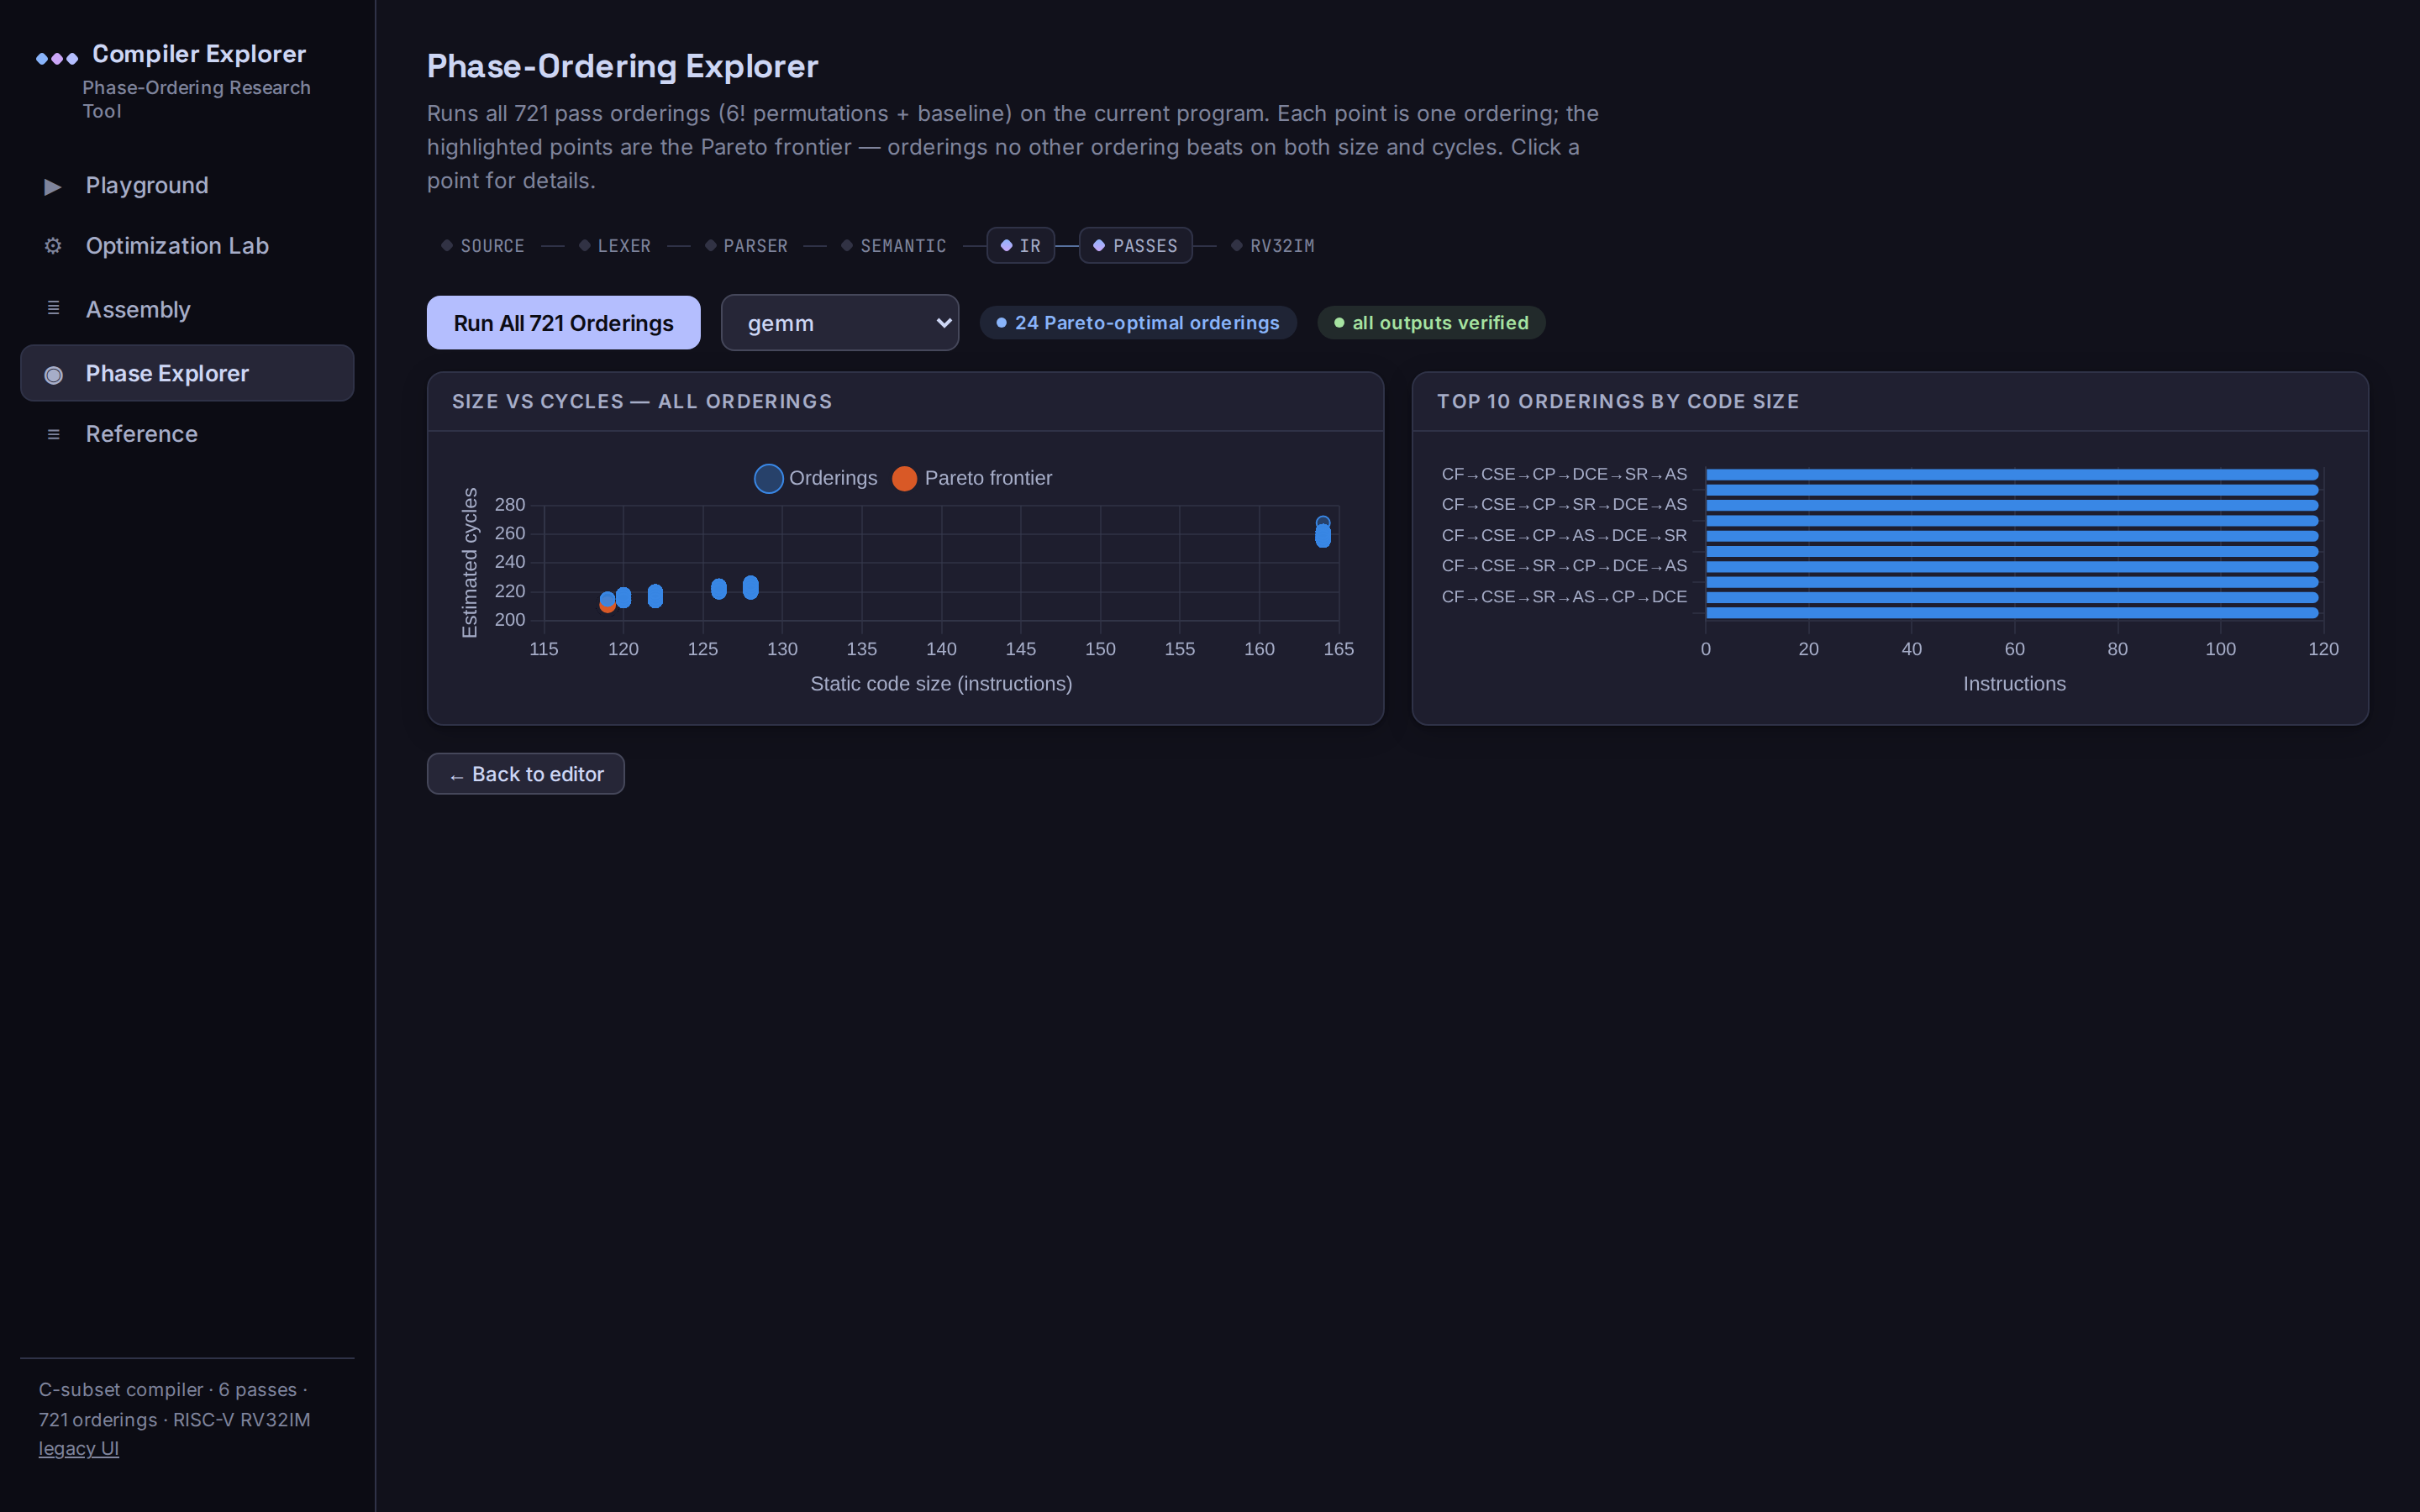
\includegraphics[width=0.82\textwidth]{gui_explorer}
\caption[Phase-Ordering Explorer page after running all 721 orderings on \code{gemm}.]{Phase-Ordering Explorer page after running all 721 orderings on \code{gemm}: size against cycles with the Pareto frontier highlighted, and the ten smallest orderings.}
\label{fig:gui-explorer}
\end{figure}

\section{Societal Impact of the Project}

The most immediate impact of the project is educational. Compiler construction is taught in every computer science programme, and optimization is the part of the course that students find most abstract, because the effects are indirect and the tools that exhibit them are too large to read. The web application turns the phase-ordering problem into something a student can manipulate in a browser within minutes: load a program, drag a pass, watch the code change. Because the whole compiler is about four thousand lines of readable Python, it also serves as a reference implementation that a student can study end to end, modify, and extend as a course project; the exhaustive results in this chapter give an instructor ground truth against which student-written passes or student-chosen orderings can be checked. The tool requires no installation beyond Python and runs offline, so it is usable in institutions with limited computing infrastructure.

The second impact is on the practice of embedded software development. India's manufacturing sector, and in particular its micro, small, and medium enterprises, increasingly builds products around low-cost microcontrollers, and the RISC-V instruction set targeted by this project's back end is becoming a common choice for such devices because it carries no licensing cost. On these devices code size determines whether a product can use a cheaper part with less flash, and executed instructions determine battery life. The study shows that on embedded-style kernels the difference between a good and a poor pass ordering is a factor of two or more in code-size reduction and a quarter of all executed instructions. A firmware team that understands this can evaluate its toolchain's options with a small effort, and the infrastructure provides a template for how such an evaluation, exhaustive, output-validated, and reported with geometric means, should be done. The longer-term prospect, identified in the future work, is an automatic ordering selector that a small manufacturer could apply without compiler expertise.

The third impact is on research practice. The project demonstrates that a complete, reproducible phase-ordering study can be carried out by an undergraduate team with a purpose-built infrastructure, and that the central phenomena reported for production compilers reproduce exactly at small scale. The repository, the benchmark suite, the results, and the tool are available for other students and researchers to build on, and the API makes the infrastructure usable as an environment for testing search and learning methods against exhaustive ground truth. Finally, the project has a modest environmental dimension: every instruction that a compiler removes from a program is energy that the program will not consume, on every device and every execution for the life of the product, and a better understanding of how to remove instructions is a small contribution to more efficient computing.

\section{SDG Mapped}

The project's objectives and outcomes align with the following United Nations Sustainable Development Goals.

\begin{itemize}
  \item \textbf{SDG 4: Quality Education.} The interactive application and the readable compiler are teaching instruments for one of the harder topics in the computer science curriculum. They are free, run offline on modest hardware, and are documented for self-study, which supports equitable access to technical education.
  \item \textbf{SDG 9: Industry, Innovation, and Infrastructure.} The project contributes tools and evidence for building more efficient embedded software on open hardware, and demonstrates a reproducible methodology for compiler evaluation that small engineering organizations can adopt. Its use of the open RISC-V architecture supports indigenous, license-free technology development.
  \item \textbf{SDG 8: Decent Work and Economic Growth.} By showing how compiler configuration affects the cost of embedded products, and by pointing towards automatic tuning that requires no compiler specialist, the project supports the productivity of micro, small, and medium enterprises that build electronic products.
  \item \textbf{SDG 7: Affordable and Clean Energy, and SDG 12: Responsible Consumption and Production (indirect).} Smaller and faster firmware consumes less energy and allows products to use smaller parts. The project quantifies one lever, pass ordering, for achieving both, and its future work targets measured energy directly.
  \item \textbf{SDG 17: Partnerships for the Goals.} The infrastructure is built on and gives back to open-source foundations, uses community benchmark suites, and is designed as a shared platform on which other institutions can run experiments and courses.
\end{itemize}
